%  LaTeX support: latex@mdpi.com
%  In case you need support, please attach all files that are necessary for compiling as well as the log file, and specify the details of your LaTeX setup (which operating system and LaTeX version / tools you are using).

%=================================================================
\documentclass[mathematics,article,submit,moreauthors,pdftex]{mdpi}

% If you would like to post an early version of this manuscript as a preprint, you may use preprint as the journal and change 'submit' to 'accept'. The document class line would be, e.g., \documentclass[preprints,article,accept,moreauthors,pdftex]{mdpi}. This is especially recommended for submission to arXiv, where line numbers should be removed before posting. For preprints.org, the editorial staff will make this change immediately prior to posting.

%% Some pieces required from the pandoc template
\providecommand{\tightlist}{%
  \setlength{\itemsep}{0pt}\setlength{\parskip}{4pt}}
\setlist[itemize]{leftmargin=*,labelsep=5.8mm}
\setlist[enumerate]{leftmargin=*,labelsep=4.9mm}

\usepackage{longtable}

% see https://stackoverflow.com/a/47122900

%--------------------
% Class Options:
%--------------------
%----------
% journal
%----------
% Choose between the following MDPI journals:
% acoustics, actuators, addictions, admsci, aerospace, agriculture, agriengineering, agronomy, algorithms, animals, antibiotics, antibodies, antioxidants, applsci, arts, asc, asi, atmosphere, atoms, axioms, batteries, bdcc, behavsci , beverages, bioengineering, biology, biomedicines, biomimetics, biomolecules, biosensors, brainsci , buildings, cancers, carbon , catalysts, cells, ceramics, challenges, chemengineering, chemistry, chemosensors, children, cleantechnol, climate, clockssleep, cmd, coatings, colloids, computation, computers, condensedmatter, cosmetics, cryptography, crystals, dairy, data, dentistry, designs , diagnostics, diseases, diversity, drones, econometrics, economies, education, electrochem, electronics, energies, entropy, environments, epigenomes, est, fermentation, fibers, fire, fishes, fluids, foods, forecasting, forests, fractalfract, futureinternet, futurephys, galaxies, games, gastrointestdisord, gels, genealogy, genes, geohazards, geosciences, geriatrics, hazardousmatters, healthcare, heritage, highthroughput, horticulturae, humanities, hydrology, ijerph, ijfs, ijgi, ijms, ijns, ijtpp, informatics, information, infrastructures, inorganics, insects, instruments, inventions, iot, j, jcdd, jcm, jcp, jcs, jdb, jfb, jfmk, jimaging, jintelligence, jlpea, jmmp, jmse, jnt, jof, joitmc, jpm, jrfm, jsan, land, languages, laws, life, literature, logistics, lubricants, machines, magnetochemistry, make, marinedrugs, materials, mathematics, mca, medicina, medicines, medsci, membranes, metabolites, metals, microarrays, micromachines, microorganisms, minerals, modelling, molbank, molecules, mps, mti, nanomaterials, ncrna, neuroglia, nitrogen, notspecified, nutrients, ohbm, particles, pathogens, pharmaceuticals, pharmaceutics, pharmacy, philosophies, photonics, physics, plants, plasma, polymers, polysaccharides, preprints , proceedings, processes, proteomes, psych, publications, quantumrep, quaternary, qubs, reactions, recycling, religions, remotesensing, reports, resources, risks, robotics, safety, sci, scipharm, sensors, separations, sexes, signals, sinusitis, smartcities, sna, societies, socsci, soilsystems, sports, standards, stats, surfaces, surgeries, sustainability, symmetry, systems, technologies, test, toxics, toxins, tropicalmed, universe, urbansci, vaccines, vehicles, vetsci, vibration, viruses, vision, water, wem, wevj

%---------
% article
%---------
% The default type of manuscript is "article", but can be replaced by:
% abstract, addendum, article, benchmark, book, bookreview, briefreport, casereport, changes, comment, commentary, communication, conceptpaper, conferenceproceedings, correction, conferencereport, expressionofconcern, extendedabstract, meetingreport, creative, datadescriptor, discussion, editorial, essay, erratum, hypothesis, interestingimages, letter, meetingreport, newbookreceived, obituary, opinion, projectreport, reply, retraction, review, perspective, protocol, shortnote, supfile, technicalnote, viewpoint
% supfile = supplementary materials

%----------
% submit
%----------
% The class option "submit" will be changed to "accept" by the Editorial Office when the paper is accepted. This will only make changes to the frontpage (e.g., the logo of the journal will get visible), the headings, and the copyright information. Also, line numbering will be removed. Journal info and pagination for accepted papers will also be assigned by the Editorial Office.

%------------------
% moreauthors
%------------------
% If there is only one author the class option oneauthor should be used. Otherwise use the class option moreauthors.

%---------
% pdftex
%---------
% The option pdftex is for use with pdfLaTeX. If eps figures are used, remove the option pdftex and use LaTeX and dvi2pdf.

%=================================================================
\firstpage{1}
\makeatletter
\setcounter{page}{\@firstpage}
\makeatother
\pubvolume{xx}
\issuenum{1}
\articlenumber{5}
\pubyear{2019}
\copyrightyear{2019}
%\externaleditor{Academic Editor: name}
\history{Received: date; Accepted: date; Published: date}
\updates{yes} % If there is an update available, un-comment this line

%% MDPI internal command: uncomment if new journal that already uses continuous page numbers
%\continuouspages{yes}

%------------------------------------------------------------------
% The following line should be uncommented if the LaTeX file is uploaded to arXiv.org
%\pdfoutput=1

%=================================================================
% Add packages and commands here. The following packages are loaded in our class file: fontenc, calc, indentfirst, fancyhdr, graphicx, lastpage, ifthen, lineno, float, amsmath, setspace, enumitem, mathpazo, booktabs, titlesec, etoolbox, amsthm, hyphenat, natbib, hyperref, footmisc, geometry, caption, url, mdframed, tabto, soul, multirow, microtype, tikz

%=================================================================
%% Please use the following mathematics environments: Theorem, Lemma, Corollary, Proposition, Characterization, Property, Problem, Example, ExamplesandDefinitions, Hypothesis, Remark, Definition
%% For proofs, please use the proof environment (the amsthm package is loaded by the MDPI class).

%=================================================================
% Full title of the paper (Capitalized)
\Title{Gráfico de control \(T^2\) Hotelling para variables cualitativas}

% Authors, for the paper (add full first names)
\Author{Wilson
Rojas-Preciado$^{1,2,*}$\href{https://orcid.org/0000-0003-1614-698X}{\orcidicon}, Mauricio
J.
Rojas-Campuzano$^{3}$\href{https://orcid.org/0000-0001-8000-9432}{\orcidicon}, Purificación
Galindo-Villardón$^{2}$\href{https://orcid.org/0000-0001-6977-7545}{\orcidicon}, Omar
Ruiz-Barzola$^{3}$\href{https://orcid.org/0000-0001-8206-1744}{\orcidicon}}

% Authors, for metadata in PDF
\AuthorNames{Wilson Rojas-Preciado, Mauricio J.
Rojas-Campuzano, Purificación Galindo-Villardón, Omar Ruiz-Barzola}

% Affiliations / Addresses (Add [1] after \address if there is only one affiliation.)
\address{%
$^{1}$ \quad Universidad Técnica de Machala - Machala,
Ecuador; \href{mailto:wrojas@utmachala.edu.ec}{\nolinkurl{wrojas@utmachala.edu.ec}}\\
$^{2}$ \quad Universidad de Salamanca Salamanca,
España; \href{mailto:wrojas@usal.es}{\nolinkurl{wrojas@usal.es}};
\href{mailto:pgalindo@usal.es}{\nolinkurl{pgalindo@usal.es}}\\
$^{3}$ \quad Escuela Superior Politécnica del Litoral Gayaquil,
Ecuador; \href{mailto:maujroja@espol.edu.ec}{\nolinkurl{maujroja@espol.edu.ec}};
\href{mailto:oruiz@espol.edu.ec}{\nolinkurl{oruiz@espol.edu.ec}}\\
}
% Contact information of the corresponding author
\corres{Correspondence: \href{mailto:wrojas@utmachala.edu.ec}{\nolinkurl{wrojas@utmachala.edu.ec}};
Tel.: +593-992-83-3719}

% Current address and/or shared authorship
\firstnote{Current address: Updated affiliation}







% The commands \thirdnote{} till \eighthnote{} are available for further notes

% Simple summary
\simplesumm{A Simple summary goes here.}

% Abstract (Do not insert blank lines, i.e. \\)
\abstract{La literatura científica es abundante en lo referente a
gráficos de control en entornos multivariantes para datos numéricos y
mixtos, sin embargo, para datos cualitativos hay pocas publicaciones.
Las variables cualitativas aportan valiosa información de procesos en
diversos contextos industriales, productivos, sociales. Los procesos
educativos no son una excepción, tienen múltiples variables asociadas a
estudiantes, profesores e instituciones. Cuando hay muchas variables se
corre el riesgo de tomar información redundante o excesiva, luego, es
viable la aplicación de métodos multivariantes de reducción de
dimensiones para quedarse con pocas variables ficticias, combinación de
las reales, que sinteticen la mayor parte de la información. En este
contexto se presenta el gráfico de control T2Qv, una técnica de control
estadístico de procesos multivariantes que realiza un análisis de datos
cualitativos mediante Análisis de correspondencias múltiples (MCA),
Análisis Factorial Múltiple y el gráfico \(T^2\) de Hotelling. La
interpretación de los puntos fuera de control se realiza comparando los
gráficos MCA y analizando la distancia \(X^2\) entre las categorías de
la tabla concatenada y las que representan puntos fuera de control. El
análisis de sensibilidad determinó que el gráfico de control T2Qv tiene
un buen rendimiento cuando trabaja con altas dimensiones. Para probar la
metodología se hizo un análisis con datos simulados y otro con datos
reales relacionados con la educación superior. Para facilitar la
difusión y aplicación de la propuesta, se desarrolló un paquete
computacional reproducible en R, denominado T2Qv y disponible en The
Comprehensive R Archive Network (CRAN).}

% Keywords
\keyword{Multivariate; Statistical Process Control; Cualitative; Control
Charts; R; T2 Hotelling; Superior Education.}

% The fields PACS, MSC, and JEL may be left empty or commented out if not applicable
%\PACS{J0101}
%\MSC{}
%\JEL{}

%%%%%%%%%%%%%%%%%%%%%%%%%%%%%%%%%%%%%%%%%%
% Only for the journal Diversity
%\LSID{\url{http://}}

%%%%%%%%%%%%%%%%%%%%%%%%%%%%%%%%%%%%%%%%%%
% Only for the journal Applied Sciences:
%\featuredapplication{Authors are encouraged to provide a concise description of the specific application or a potential application of the work. This section is not mandatory.}
%%%%%%%%%%%%%%%%%%%%%%%%%%%%%%%%%%%%%%%%%%

%%%%%%%%%%%%%%%%%%%%%%%%%%%%%%%%%%%%%%%%%%
% Only for the journal Data:
%\dataset{DOI number or link to the deposited data set in cases where the data set is published or set to be published separately. If the data set is submitted and will be published as a supplement to this paper in the journal Data, this field will be filled by the editors of the journal. In this case, please make sure to submit the data set as a supplement when entering your manuscript into our manuscript editorial system.}

%\datasetlicense{license under which the data set is made available (CC0, CC-BY, CC-BY-SA, CC-BY-NC, etc.)}

%%%%%%%%%%%%%%%%%%%%%%%%%%%%%%%%%%%%%%%%%%
% Only for the journal Toxins
%\keycontribution{The breakthroughs or highlights of the manuscript. Authors can write one or two sentences to describe the most important part of the paper.}

%\setcounter{secnumdepth}{4}
%%%%%%%%%%%%%%%%%%%%%%%%%%%%%%%%%%%%%%%%%%

% Pandoc citation processing

\usepackage{subfig}

\begin{document}
%%%%%%%%%%%%%%%%%%%%%%%%%%%%%%%%%%%%%%%%%%

\hypertarget{introduction}{%
\section{Introduction}\label{introduction}}

El control estadístico juega un rol muy importante en la mejora continua
de los procesos y dentro de éste, los gráficos de control, los cuales
ayudan a monitorizar los procesos, han sido extensamente utilizados
desde su creación por Walter Shewhart \citep{Gutierrez2013} hasta
nuestros días. A partir de los gráficos univariantes se han desarrollado
un sinnúmero de propuestas, las cuales incorporaron la opción de
monitorizar varias variables a la vez \citep{ramos2017, li2012},
abriendo con ello el control estadístico de procesos multivariantes
(CEPM).

Las opciones más conocidas en el CEPM son: El gráfico de control T2 de
Hotelling \citep{hotelling1947}, el cual se podría considerar la versión
multivariante del gráfico de medias de Shewhart; el MEWMA
\citep{lowry1992}, el cual es la versión multivariante del gráfico de
medias ponderadas EWMA \citep{roberts2000control}; o el MCUSUM
\citep{Crosier1988}, el cual es la versión multivariante del grafico de
control de sumas acumuladas CUSUM \citep{page1954continuous}.

A estos gráficos de control multivariante se le han realizado varias
mejoras tales como: su optimización, determinando de forma analítica
\citep{Aparisi1996, Aparisi2001, Faraz2006} o heurística los valores
óptimos de sus parámetros \citep{ruiz2013}; otra propuesta es la de
trabajar sin distribuciones probabilísticas o versiones no paramétricas
\citep{shabbak2012, liu2020, xue2020}, para procesos continuos o por
lotes \citep{ramos2017}.

Todos estos gráficos de control multivariantes tienen un enfoque
cuantitativo; es decir, las variables monitorizadas son esencialmente
cuantitativas, ya sean discretas o continuas. Para ello, los diferentes
autores, inicialmente se valieron de la distancia de Mahalanobis
\citep{mahalanobis1936generalised}. Posteriormente, para el análisis de
una combinación de variables continuas y categóricas se desarrolló el
gráfico basado en la distancia de Gower \citep{Tuerhong2014}. Sin
embargo, el abordaje de problemas como la alta correlación entre
características y en presencia de datos mixtos, requirió la
incorporación de técnicas estadísticas multivariantes clásicas, como
Análisis de Componentes Principales \citep{pearson1901liii}, Métodos
Biplot \citep{gabriel1971biplot, galindojk}, Análisis de
correspondencias \citep{Benzecri}, STATIS
\citep{l1976structuration, robert1976unifying, lavit1988presentation},
Coordenadas paralelas \citep{inselberg1990parallel}, Análisis de
conglomerados \citep{edwards1965method}.

Dentro de las aportaciones referentes a los gráficos de control que
incorporan técnicas multivariantes destacan el gráfico basado en STATIS
para el monitoreo de procesos por lotes en entornos no paramétricos
\citep{filho2016multivariate}; los diagramas de bolsa robustos que
utilizan STATIS Dual y Coordenadas paralelas \citep{RamosBarberan2018};
el Gráfico de control multivariante PCA para datos mixtos, que aplica
una combinación de Análisis de Componentes Principales y Análisis de
Correspondencias Múltiples \citep{Muhammad2018}; el gráfico de control
de peso de novedad sensible a la densidad (DNW) utiliza el algoritmo
\(k\)-vecino más cercano (kNN) \citep{liu2020}; el gráfico basado en
Kernel PCA Mix \citep{Ahsan2020, Ahsan2022}; el Gráfico \(T^2\) basado
en la combinación de PCA para datos continuos y cualitativos con
detección de datos atípicos \citep{Ahsan2021}; los gráficos de control
basados en PCA para entornos no paramétricos
\citep{Farokhnia, liu2020nonparametric}.

No obstante, las aportaciones al desarrollo de gráficos de control
multivariante para variables cualitativas no han sido numerosas. En este
campo las propuestas se han desarrollado alrededor del análisis de
variables que siguen una distribución Poisson y el análisis de variables
multinomiales. La primera propuesta fue la de \citet{holgate1964}, quien
presentó un trabajo sobre la distribución Poisson bivariante para
variables correlacionadas. Este modelo fue tomado como insumo en las
investigaciones de autores como \citet{chiu2007}, \citet{ho2009},
\citet{laungrungrong2011ewma}, \citet{epprecht2013optimal}.

Otra propuesta destacada es la de \citet{lu1998control}, quien
desarrolló un gráfico de control tipo Shewhart para procesos
multivariantes con variables cualitativas, cuando la característica de
calidad asume valores binarios, al cual denominaron gráfico np
multivariante (MNP). Ya en el contexto multinomial,
\citet{ranjan2008multivariate} planteó un gráfico de control
multivariante utilizando el estadístico \(D^2\) de Mahalanobis para
atributos que siguen una distribución multinomial. Además, de una
propuesta para procesos multinomiales bajo el enfoque difuso
\citep{taleb2006multivariate}; \citet{taleb2009control} introdujo
gráficos de control para el monitoreo de procesos multivariados con
datos lingüísticos multidimensionales, basados en dos procedimientos: la
teoría de la probabilidad y la teoría difusa;
\citet{pastuizaca2015multivariate} presentaron un gráfico de control
multivariante multinomial T2 con un enfoque difuso.

\citet{Saltos2020} aseguran que las herramientas de control de la
calidad se pueden considerar no solo para monitorizar procesos
industriales sino también procesos relacionados con la educación, por
ejemplo, la evaluación del desempeño estudiantil. Estos autores
aplicaron el concepto de profundidad, que transforma una observación
multivariante a un índice univariante, el cual es susceptible de
monitorizar en una carta de control y para esto utilizaron la carta r,
además utilizaron clúster medio para establecer umbrales que faciliten
la conformación de grupos y establecer perfiles de estudiantes mediante
medidas descriptivas.

En el estudio de los procesos que se desarrollan en el entorno social se
maneja con mucha frecuencia variables cualitativas. No es que estén
ausentes los datos cuantitativos, sino que, en las bases de datos que se
utilizan para estos análisis, abundan las variables cualitativas
nominales y ordinales, a veces, sobre las de tipo numérico.

\citet{perez2004} señala que al observar muchas variables sobre una
muestra es presumible que una parte de la información recogida pueda ser
redundante o que sea excesiva, en cuyo caso los métodos multivariantes
de reducción de la dimensión tratan de eliminarla combinando muchas
variables observadas para quedarse con pocas variables ficticias que,
aunque no observadas, sean combinación de las reales y sinteticen la
mayor parte de la información contenida en sus datos. En este caso se
deberá tener en cuenta el tipo de variables que maneja. Si son variables
cuantitativas las técnicas que le permiten este tratamiento pueden ser
el Análisis de componentes principales
\citep{Person1901, Hotelling1933}, el Análisis factorial
\citep{ch1904, thurstone1947, kaiser1958}, mientras que, si se trata de
variables cualitativas, es recomendable la aplicación de un Análisis de
correspondencias múltiple, Análisis de homogeneidad o un Análisis de
Escalamiento multidimensional.

En el control estadístico de procesos, los aportes al desarrollo de
gráficos de control para variables cualitativas todavía son incipientes,
las pocas publicaciones se orientan al análisis de características de la
calidad en procesos industriales, pero no a procesos sociales. Al
analizar los procedimientos publicados por los autores citados en este
estudio, se detectan limitaciones que podrían restringir su aplicación,
por ejemplo, el análisis de pocas características de la calidad, el uso
de muestras constituidas por elementos individuales en vez de grupos, la
dificultad de trabajar con muchas categorías de forma simultánea. Surge,
entonces, la necesidad de un gráfico de control para la representación
de p variables cualitativas, que pueda trabajar con múltiples categorías
nominales y ordinales y que facilite la identificación de las causas que
pueden llevar al proceso a un estado fuera de control y que pueda ser
aplicado en procesos sociales.

El presente artículo atiende las limitaciones antes mencionadas en
cuanto a gráficos de control para variables cualitativas y su aplicación
en un entornos sociales. Por tal motivo, su objetivo es desarrollar un
gráfico de control para variables cualitativas mediante el uso de
metodologías estadísticas multivariantes, para que se contribuya a la
diversificación de técnicas en la fase I del control estadístico de
procesos.

Este artículo está organizado de la siguiente manera: la Introducción,
que establece los antecedentes conceptuales y referenciales de los
gráficos de control multivariantes aplicados a variables cualitativas;
la sección 2, materiales y métodos, que detalla el procedimiento que se
siguió en el desarrollo del gráfico de control propuesto; la sección 3
describe al complemento computacional que facilita la aplicación de esta
metodología; la sección 4 muestra los resultados mediante el análisis de
datos simulados; la sección 5 corresponde al análisis de sensibilidad
que relaciona el número de dimensiones analizadas versus la
confiabilidad de los resultados. La sección 6 presenta la discusión
mediante un análisis comparativo entre el gráfico de control T2Qv y las
propuestas de otros autores. Finalmente, la sección 7 establece las
conclusiones.

\hypertarget{metodologuxeda}{%
\section{Metodología}\label{metodologuxeda}}

\hypertarget{notaciuxf3n}{%
\subsection{Notación}\label{notaciuxf3n}}

La tabla \ref{tab:notacion} contiene elementos, representación y
ejemplos de la manera como se presentan los elementos algebraicos
abordados en la metodología.

\begin{table}[!ht]
\begin{center}
 \begin{tabular}{||c ||c |c ||} 
 \hline
 Elementos & Representación & Ejemplo \\
 \hline\hline
 Escalares & Letras en minúscula. & $v,\lambda$\\
\hline
Vectores & Letras en minúscula y en negrita. & $\mathbf{v},\mathbf{u}$\\
\hline
Matrices & Letras en mayúscula y en negrita. & $\mathbf{V},\mathbf{X}$\\
\hline
Matrices de tres vías (Cubos de datos) & Letras con doble trazo en mayúscula. & $\mathbb{C},\mathbb{X}$\\
\hline
\end{tabular}\caption{Elementos algebraicos}
\label{tab:notacion}
\end{center}
\end{table}

A lo largo del artículo se utilizarán letras para hacer referencia a
parámetros necesarios, se los enuncia a continuación en la tabla
\ref{tab:notacion2}:

\begin{table}[!ht]
\begin{center}
 \begin{tabular}{||c ||c | c ||} 
 \hline
 Letra &  Significado & Especificación\\
 \hline\hline
 $p$ & Número de dimensiones &\\
\hline
 $K$ & Número total de tablas (Especifica la profundidad del cubo de datos) & \\
 \hline
 $k$ & Índice de tabla &  k=1,2,...,K\\
  \hline
 $T$ & Índice de matriz transpuesta &  $\mathbf{X^{T}}$\\
\hline
 $n$ & Tamaño muestral de las $k$ tablas &\\
\hline
\end{tabular}\caption{Notación}
\label{tab:notacion2}
\end{center}
\end{table}

\hypertarget{anuxe1lisis-de-correspondencias-muxfaltiples-mca}{%
\subsection{Análisis de Correspondencias Múltiples
(MCA)}\label{anuxe1lisis-de-correspondencias-muxfaltiples-mca}}

Dado que se trabaja con variables cualitativas se aplica Análisis de
Correspondencias \citep{Benzecri} analizando la similaridad entre
categorías \citep{perez2004} basada en la distancia \(\chi^2\), siendo
este un análisis similar al de componentes principales.

En este caso no se aplica el enfoque francés \citep{michailidis1998}, si
no el anglosajón, donde el MCA se denomina Análisis de Homogeneidad o
Escalamiento Dual, haciendo uso de la tabla de Burt \citep{Benzecri} y
partiendo de una matriz de datos con p variables cualitativas, cada una
con \(h\) categorías \((h >1)\). La matriz compuesta por las \(n\) filas
u observaciones y las \(p\) columnas o variables, donde cada celda
contine una de las categorías antes mencionadas, es equivalente a la
matriz disyuntiva \textbf{Z}, que desglosa las variables en cada una de
sus modalidades y registra la ocurrencia de eventos de forma binaria
\citep{Benzecri}.

La tabla de Burt viene dada por:

\begin{equation}
\mathbf{B}=\mathbf{Z'}\mathbf{Z}
\label{eq:Burt}
\end{equation}

La matriz B en \ref{eq:Burt} está formada por las frecuencias absolutas,
éstas se transforman en frecuencias relativas, dividiendo los valores de
la matriz por la frecuencia total, dando lugar a la matriz \textbf{P}.

Se obtienen los vectores de \emph{Masas de fila (mf)} y \emph{columna
(mc)}, a través de las marginales de las filas y de las columnas de la
matriz \textbf{P}, respectivamente.

Se obtiene la matriz de residuos estandarizados \textbf{S}.

\begin{equation}
\mathbf{S}=\mathbf{D_{fila}}^{-\frac{1}{2}}(\mathbf{P}-\mathbf{mf} \hspace{0.2cm} \mathbf{mc'})\mathbf{D_{columna}}^{-\frac{1}{2}}
\label{eq:s}
\end{equation}

donde \(\mathbf{D_{fila}}\) es una matriz diagonal que contiene las
masas de las filas y \(\mathbf{D_{columna}}\) es una matriz diagonal que
contiene las masas de las columnas.

Se aplica descomposición singular (SVD) a la matriz \textbf{S} (Ecuación
\ref{eq:s}):

\begin{equation}
\mathbf{S}=\mathbf{U}\mathbf{D}\mathbf{V'}
\label{eq:svd}
\end{equation}

donde \(\mathbf{U}\) y \(\mathbf{V}\) son matrices ortogonales y
\(\mathbf{D}\) es una matriz diagonal que contiene los valores
singulares.

Luego se obtienen las coordenadas estandarizadas, para lo cual se
aplican las ecuaciones \ref{eq:xcoor} y \ref{eq:ycoor}. \begin{equation}
\mathbf{X}=\mathbf{D_{fila}}^{-\frac{1}{2}} \mathbf{U}
\label{eq:xcoor}
\end{equation}

\begin{equation}
\mathbf{Y}=\mathbf{D_{columna}}^{-\frac{1}{2}} \mathbf{V}
\label{eq:ycoor}
\end{equation}

\hypertarget{generalizaciuxf3n-a-k-tablas}{%
\subsubsection{\texorpdfstring{Generalización a \(k\)
tablas}{Generalización a k tablas}}\label{generalizaciuxf3n-a-k-tablas}}

Si se tienen \emph{K} tablas, de igual estructura y compuestas por
variables cualitativas, a cada una de las \emph{K} tablas se aplica lo
descrito en 2.2, obteniéndose el conjunto de \(K\) tablas con formato
inicial \ref{tab:inicial}.

\begin{figure}[!ht]


\begin{center}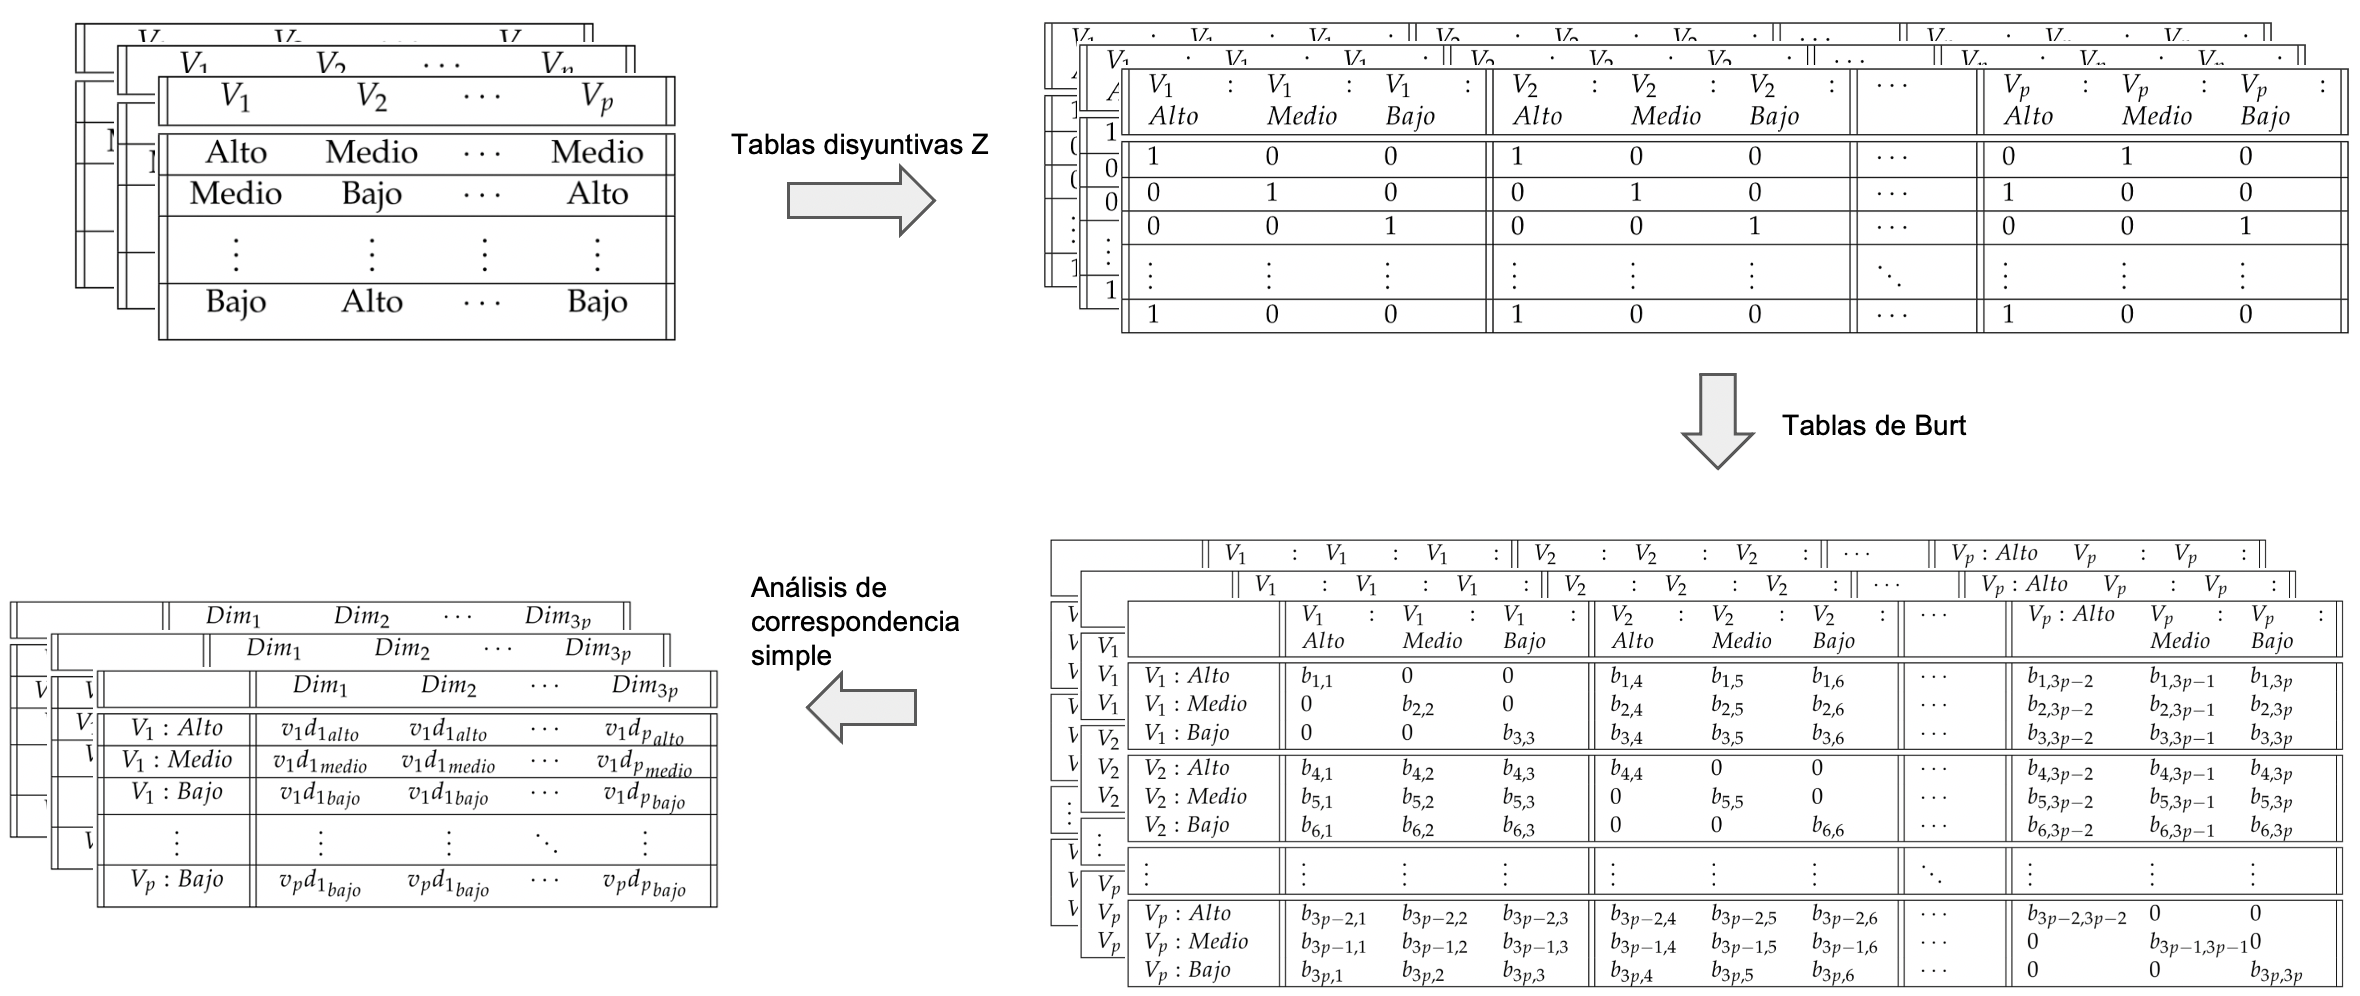
\includegraphics[width=0.9\linewidth,]{ktablesMCA} \end{center}

\caption{Procedimiento del MCA para $k$ tablas}

\label{fig:MCAk}
\end{figure}

Se denomina \(C\) a cada una de las \(K\) tablas de coordenadas
obtenidas en el paso anterior. Con la finalidad de detectar la magnitud
de las variables latentes, se aplica valor absoluto a los elementos de
la matriz \(C_{k} (k=1,…, K)\). De esta forma se obtiene un conjunto de
\emph{k} tablas de coordenadas (cargas), cuyas filas corresponden a las
variables observadas y las columnas a las variables latentes.

\hypertarget{normalizaciuxf3n-de-tablas}{%
\subsubsection{Normalización de
tablas}\label{normalizaciuxf3n-de-tablas}}

A las \(K\) tablas \textbf{C} se le aplica la normalización \citep{AFM}
del Análisis factorial múltiple (MFA).

Sea \(\lambda_{1}^{k}\) el primer valor propio obtenido de la
descomposición singular de la \(k\)-ésima tabla \textbf{C}. Se normaliza
la tabla multiplicándola por \(1/\lambda_{1}^{k}\). Con esto se obtiene
la tabla \(C^{'}\), que corresponde a la tabla de coordenadas
normalizadas.\\
Individualmente, para el caso de la matriz \(k\), se tendría la
siguiente expresión.

\begin{equation}
\mathbf{C'_k}=\frac{1}{\lambda_{k}^1} \mathbf{C_k}
\label{eq:Cprimak}
\end{equation}

Hasta este punto se tiene un conjunto de matrices de coordenadas
normalizadas, cuyas filas contienen las variables observadas y las
columnas, las variables latentes.

La expresión de la ecuación \ref{eq:Cprimak} aplicada a k tablas se
representa en la figura \ref{fig:esquema1}, que muestra el esquema de
preparación de las tablas, previo a la obtención de vectores de
centralidad usados por el gráfico de control multivariante.

Unificando las \emph{K} tablas normalizadas \(C^{'}\) en una sola, se
tiene la matriz \(\mathbb{C}^{'}\), denominada Matriz Concatenada. Esta
contiene todos los elementos de las \emph{K} tablas normalizadas.

\begin{equation}
\mathbf{\mathbb{C^{'}}}=[\mathbf{C_1^{'}}|\mathbf{C_2^{'}}|,...,|\mathbf{C'_{K}}]^{T}
\label{eq:Cprima}
\end{equation}

La normalización que realiza el MFA se encarga de ponderar las \emph{K}
tablas, con el objetivo de evitar alguna descompensación al momento de
realizar el análisis conjunto de las tablas.

A partir de las matrices \(\mathbf{\mathbb{C^{'}}}\) y
\(\mathbf{C_k^{'}}\), se obtiene los vectores de mediana, tal como se
muestra en la figura \ref{fig:esquema2}. El vector
\(\mathbf{\tilde{x}_{C_k^{'}}}\) explicará el comportamiento central de
la tabla k y el vector \(\mathbf{\tilde{x}_{\mathbb{C^{'}}}}\) explicará
el comportamiento de la matriz concatenada.

\begin{figure}[!h]


\begin{center}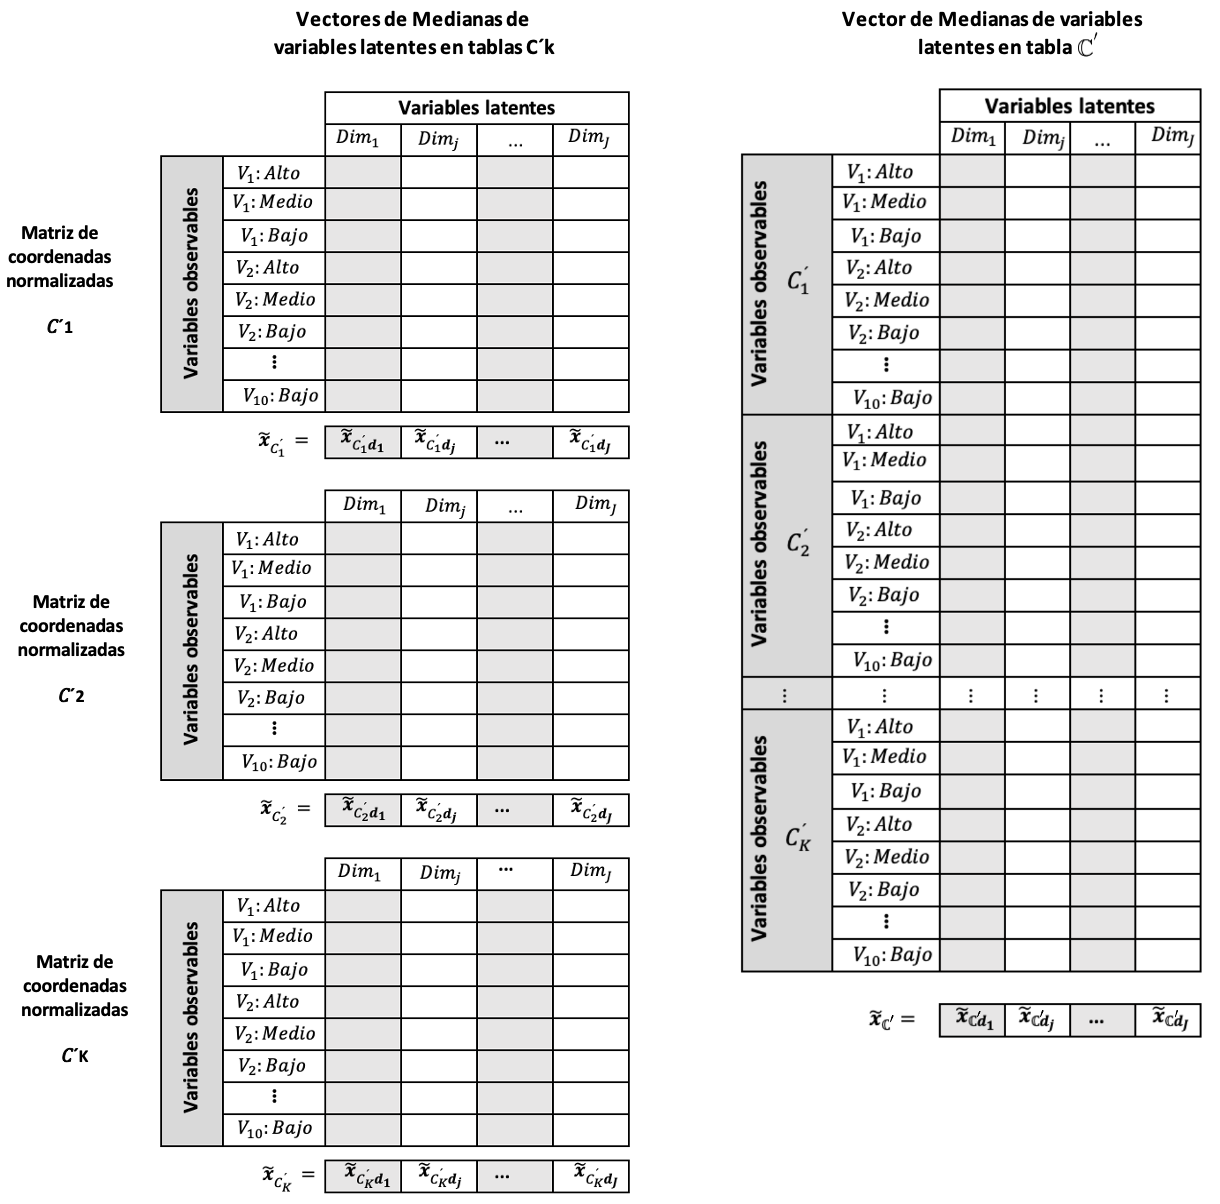
\includegraphics[width=0.9\linewidth,]{esquema_2} \end{center}

\caption{Esquema de obtención de vectores de medianas}

\label{fig:esquema2}
\end{figure}

\hypertarget{gruxe1fico-de-control-t2qv}{%
\subsection{Gráfico de control T2Qv}\label{gruxe1fico-de-control-t2qv}}

\hypertarget{obtenciuxf3n-del-gruxe1fico-de-control}{%
\subsubsection{Obtención del gráfico de
control}\label{obtenciuxf3n-del-gruxe1fico-de-control}}

Para definir el gráfico de control \(T^2\) Hotelling se deben tomar las
siguientes consideraciones:

\begin{itemize}
\tightlist
\item
  La tabla \(\mathbb{C}^{'}\) (Ecuación \ref{eq:Cprima}) se denomina
  Concatenada, sirve como referente para el escenario \emph{bajo
  control} en la fase I del control del proceso.
\item
  El estadístico \(T^2\) Hotelling normalmente se calcula con los
  vectores de media y la matriz de covarianzas del proceso bajo control;
  la propuesta de esta investigación es adoptar conceptos de robustez,
  utilizando el vector de medianas en vez de el vector de medias, en
  virtud de que a las medianas no les afectan los valores atípicos.
\item
  De la matriz concatenada \(\mathbb{C}^{'}\) se obtiene
  \(\tilde{x_{0}}\) (Vector de medianas de la matriz concatenada) y
  \(S_0\) (Matriz de covarianzas de la matriz concatenada).
\item
  Cada matriz \(\mathbf{C'_k}\) tiene el mismo número de columnas.
\item
  El vector de medias \(\tilde{x_{k}}\) está atado a la tabla
  \(\mathbf{C'_k}\), es decir, el gráfico de control estará en función
  de las diferencias entre las matrices \(\mathbf{C'_k}\) y la matriz
  concatenada \(\mathbf{\mathbb{C^{'}}}\).
\item
  Las matrices \(\mathbf{C'_k}\) siguen una distribución normal
  multivariante con vector de mediana \(\tilde{x_{k}}\) y matriz de
  covarianzas \(\mathbf{S_k}\).
\end{itemize}

El estadístico \(T^2\) viene dado por:

\begin{equation}
T^2=n (\mu_{k}-\mu_{0})'\mathbf{\Sigma_{0}^{-1}}(\mu_{k}-\mu_{0})
\label{eq:T2}
\end{equation}

Tomando en cuenta las consideraciones previas, se obtiene el estadístico
\(T^2_{med}\)

\begin{equation}
T^2_{med}=n (\tilde{x_{k}}-\tilde{x_{0}})'\mathbf{\Sigma_{0}^{-1}}(\tilde{x_{k}}-\tilde{x_{0}})
\label{eq:T2med}
\end{equation}

Se sabe que, bajo control, el \(T^2\) se distribuye como una
Chi-cuadrado con \(p\) grados de libertad \(\chi^2_p\). En este caso se
puede aplicar este principio, ya que se utiliza la matriz concatenada
(\(\mathbb{C}^{'}\)), que representa al escenario bajo control.

Dado que este gráfico de control está basado en distancias de
Mahalanobis ponderadas, sólo tiene límite de control superior. Este
viene dado por la ecuación \ref{eq:UCL}

\begin{equation}
UCL=\chi^2_{\alpha,p}
\label{eq:UCL}
\end{equation}

donde \(p\) es el número de dimensiones y \(\alpha\) es la significancia
predeterminada, se considera \(\alpha=0.0027\).

\begin{figure}[!h]


\begin{center}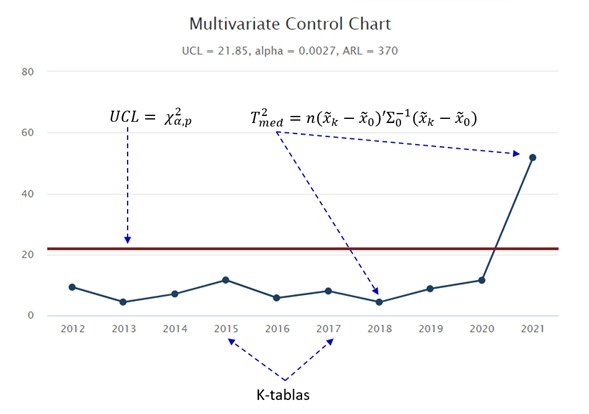
\includegraphics[width=0.7\linewidth,]{t2qvesq} \end{center}

\caption{Gráfico T2Qv}

\label{fig:t2qvesq}
\end{figure}

\hypertarget{interpretaciuxf3n-de-puntos-fuera-de-control}{%
\subsubsection{Interpretación de puntos fuera de
control}\label{interpretaciuxf3n-de-puntos-fuera-de-control}}

El gráfico multivariante para variables cualitativas, T2Qv, es capaz de
señalar que el proceso salió de control, pero no permite reconocer las
causas por las que ocurrió esto. Cada punto representado en el gráfico
representa a una tabla (muestra), constituida por un grupo de individuos
(observaciones) y \emph{p} variables que pueden tener muchas categorías,
algunas de éstas pueden mostrar un comportamiento anómalo. Por
consiguiente, es necesario analizar con detenimiento que está pasando
con los datos de las tablas reportadas para identificar la(s)
variable(s) que generaron que el proceso se salga de control.

Este análisis se realiza comparando la ubicación de los puntos que
representan las categorías de las variables en el MCA de la tabla
concatenada y la ubicación de los puntos en los gráficos MCA de cada
tabla reportada como fuera de control. Las categorías que están
incidiendo en el estado fuera de control son aquellas que muestran
diferencias notorias en su ubicación al comparar ambas tablas. Para
cuantificar la magnitud de dichas diferencias o del comportamiento
anómalo de estas categorías se calcula las distancias Chi-cuadrado entre
las masas de las columnas de la tabla reportada como fuera de control y
las columnas de la tabla concatenada, tomada esta última como referente.
Mientras mayor es el valor del estadístico, mayor es su incidencia en el
desplazamiento de la centralidad del proceso que, finalmente, pueden
llevarlo a un estado fuera de control.

\hypertarget{complemento-computacional}{%
\section{Complemento computacional}\label{complemento-computacional}}

Para facilitar la difusión y aplicación del método propuesto, se ha
desarrollado un paquete reproducible en R. El paquete \textbf{T2Qv}
\citep{T2Qv} realiza el análisis de control de \emph{K} tablas por medio
de gráficos de control multivariantes para variables cualitativas,
utilizando los fundamentos teóricos del análisis de correspondencias
múltiples y el análisis factorial múltiple, así como la idea conceptual
del STATIS.

Los gráficos se pueden mostrar de forma plana o interactiva, de la misma
manera todas las salidas se pueden mostrar en un panel interactivo de
Shiny y sus resultados gráficos y numéricos pueden ser exportados.

\hypertarget{descripciuxf3n-del-paquete-t2qv}{%
\subsection{Descripción del paquete
T2Qv}\label{descripciuxf3n-del-paquete-t2qv}}

El paquete estadístico T2Qv realiza Análisis de Correspondencias
Múltiples a las tablas originales (\(\mathbf{T_k}\)), generando matrices
de variables latentes (\(\mathbf{C_k}\)) cuyas coordenadas se someten a
un proceso de normalización, multiplicándolas por \(1/\lambda_{1}^{k}\).
Las matrices de coordenadas normalizadas (\(\mathbf{T'_k}\)) se ordenan
una debajo de otra, para conformar una tabla concatenada
(\(\mathbb{C}^{'}\)), de la que se extrae su vector de medianas
\(\tilde{\tilde{\mathbf{x}_{\mathbb{C'}}}}\) así como los vectores de
medianas de cada matriz
\(\tilde{\tilde{\mathbf{x}_{\mathbf{C'_{k}}}}}\)) que la conforman. Con
estos vectores se obtienen los estadísticos
\(T^2_{med}=n (\tilde{x_{k}}-\tilde{x_{0}})'\mathbf{\Sigma_{0}^{-1}}(\tilde{x_{k}}-\tilde{x_{0}})\)
para cada una de las tablas analizadas, los que se representan como
puntos en el gráfico de control T2Qv. Los puntos que en el gráfico se
ubiquen fuera del límite (\(UCL= \chi_{\alpha,p}^2\)) son reportados
fuera de control.

El paquete estadístico T2Qv permite la interpretación del comportamiento
anómalo de los puntos fuera de control a través de la comparación de los
gráficos MCA de una tabla \(\mathbf{TC_k}\), que resulta de concatenar
las matrices iniciales, y cada tabla inicial \(\mathbf{T'_k}\). El
paquete permite la selección de las \(\mathbf{T'_k}\). tablas, de manera
que el investigador pueda enfocar su análisis en las que se identifiquen
como fuera de control.

Además, el paquete T2Qv genera un gráfico interactivo de barras que
representa las distancias \(\chi^2\) entre las masas de columnas de las
variables de la tabla \(\mathbf{TC_k}\) y la tabla \(\mathbf{T'_k}\).
Las barras que denotan mayor altura identifican a las variables que
están provocando, con mayor fuerza, la salida de control de la
\(k\)-ésima tabla. Este gráfico interactivo incluye, mediante un gráfico
circular anidado, una representación de la distribución de las
categorías de la variable observada, correspondiente a la \(k\)-ésima
tabla, así como un gráfico circular de la distribución de las categorías
de la tabla concatenada (\(\mathbf{TC_k}\)), lo que facilita la
identificación de los cambios en la distribución de las categorías.

De esta manera el paquete T2Qv consolida la metodología propuesta en
esta investigación y permite la explicación de cuándo y por qué el
proceso salió de control.

Las funciones que incluye el paquete y su descripción se enuncian en la
tabla \ref{tab:functions}.

\begin{table}[h!]
\begin{center}
 \begin{tabular}{||c  m{35em}||} 
 \hline
  Función & Descripción \\ [0.5ex] 
 \hline\hline
 T2 qualitative & Multivariate control chart T2 Hotelling applicable for qualitative variables.\\
 \hline
  MCAconcatenated & Multiple correspondence analysis applied to a concatenated table.\\
\hline
  MCApoint & Multiple correspondence analysis applied to a specific table.\\
\hline
  ChiSq variable & Contains Chi square distance between the column masses of the table specified in PointTable and the concatenated table. It allows to identify which mode is responsible for the anomaly in the table in which it is located. \\ [1ex] 
  \hline
  Full Panel & A shiny panel complete with the 
  multivariate control chart for 
  qualitative variables, the two MCA 
  charts and the modality distance table. 
  Within the dashboard, arguments such as 
  type I error and dimensionality can be 
  modified. \\ [1ex] 
 \hline
\end{tabular}\caption{Funciones del paquete T2Qv}
\label{tab:functions}
\end{center}
\end{table}

\hypertarget{disponibilidad}{%
\subsection{Disponibilidad}\label{disponibilidad}}

El paquete está disponible en el repositorio oficial de R, The
Comprehensive R Archive Network (CRAN), la descarga se la puede realizar
de la siguiente forma:

\begin{verbatim}
install.packages("T2Qv")
\end{verbatim}

\hypertarget{resultados}{%
\section{Resultados}\label{resultados}}

Con la intención de probar la metodología propuesta en el gráfico de
control \(T^2\) de Hotelling para variables cualitativas, se hizo un
análisis con datos simulados y otro con datos reales aplicados al
contexto de la educación superior. Los resultados se obtienen de la
aplicación del paquete T2Qv.

\hypertarget{resultados-con-datos-simulados}{%
\subsection{Resultados con datos
simulados}\label{resultados-con-datos-simulados}}

\hypertarget{generaciuxf3n-de-datos-simulados}{%
\subsubsection{Generación de datos
simulados}\label{generaciuxf3n-de-datos-simulados}}

\label{simulados}

Para este estudio se generó una base de datos simulados, a la que se
denominó \emph{Datak10Contaminated}. Consta de 10 tablas, cada una de
ellas está constituida por 100 filas (observaciones) y 11 columnas, de
las cuales, las 10 primeras corresponden a las variables analizadas (V1,
V2, \ldots; V10), mismas que contienen 3 categorías (Alto, Medio y
Bajo), mientras que, la columna 11, denominada \emph{GroupLetter},
contiene el factor de clasificación de los grupos. Para su
identificación, las tablas han sido denominadas con las letras del
alfabeto, desde la \emph{a} hasta la \emph{j}. La tabla \emph{j} tiene
una distribución distinta de la que tienen las otras nueve. Las 9
primeras tablas tienen sus 10 variables con la siguiente distribución:

\[ u \sim U[0,1]\]

\[t_{1,..,9}= \left\{ \begin{array}{lcc}
             Bajo &   si  & u \leq 1/3 \\
             \\ Medio &  si & 1/3 < u < 2/3 \\
             \\ Alto &  si  & u \geq 2/3 
             \end{array}
   \right. \]

La tabla j o tabla 10, en todas sus 10 variables, sigue la distribución
presentada a continuación:

\[ u \sim U[0,1]\]

\[t_{j}= \left\{ \begin{array}{lcc}
             Bajo &   si  & u \leq 1/5 \\
             \\ Medio &  si & 1/5 < u < 2/6 \\
             \\ Alto &  si  & u \geq 2/6 
             \end{array}
   \right. \]

La base de datos se presenta en el formato establecido en la tabla
\ref{tab:tabladatos}.

\begin{table}[!ht]
\tiny
\centering
\resizebox{13cm}{!} {
\begin{tabular}{@{}lllllllllll@{}}
\toprule
\textbf{V1}                  & \textbf{V2}                    & \textbf{V3}                  & \textbf{V4}                    & \textbf{V5}                  & \textbf{V6}                    & \textbf{V7}                    & \textbf{V8}                    & \textbf{V9}                    & \textbf{V10}                   & \textbf{GroupLetter}      \\ \midrule
Low      & Medium     & Medium                       & High                           & High                         & High                           & Low                            & Medium                         & Medium                         & Medium                         & a                         \\
Low                          & Low                            & High                         & Low                            & Medium                       & High                           & High                           & High                           & Low                            & High                           & a \\
High & Medium & High & Low    & High & Medium & Medium & High   & Medium & Low    & a                         \\
Medium                       & Medium                         & Low                          & High                           & Low                          & Medium                         & High                           & Low                            & Low                            & High                           & a \\
Low  & Low    & Low  & High   & Low  & High   & High   & High   & Medium & Medium & a                         \\
High                         & High                           & Medium                       & Low                            & High                         & Low                            & Medium                         & Medium                         & High                           & Low                            & a \\
High & High   & Low  & Low    & Low  & Medium & High   & Medium & Medium & High   & a                         \\
Medium                       & Medium                         & High                         & Medium                         & Medium                       & High                           & Medium                         & High                           & High                           & High                           & a \\
Low  & Low    & Low  & Medium & High & Medium & Low    & Medium & Low    & Low    & a                         \\
Medium                       & Medium                         & Medium                       & High                           & Low                          & Medium                         & High                           & Low                            & High                           & Medium                         & a \\ \bottomrule
\end{tabular}
}

\caption{Sección de la base de datos $Datak10Contaminated$.}

\label{tab:tabladatos}

\end{table}

Para verificar la diferencia entre las distribuciones de la tabla 10 y
las demás, se calculó el promedio de las frecuencias relativas en las
tres categorías, desde la tabla \emph{a} hasta la \emph{i}, para las 10
variables (Anexo 1), luego se calculó el promedio de las frecuencias
relativas medias de las 10 variables, el resultado permite comparar la
distribución de las categorías de la tabla \emph{Datak10Contaminated}
con la distribución teórica uniforme, como se observa en la tabla
\ref{tab:tablapromfreq}.

\begin{table}[H]
\centering
\begin{tabular}{rccc}
\hline
\toprule

\textbf{Categorías} & \textbf{Teórica uniforme} & \textbf{Promedio Tablas $a$, $b$, ...,  $i$} & \textbf{Promedio Tabla $j$} \\ \midrule
\textbf{High}       & 0.333            & 0.340                & 0.724            \\ 
\textbf{Medium}     & 0.333            & 0.336                & 0.092            \\ 
\textbf{Low}        & 0.333            & 0.324                & 0.184            \\ \midrule
\end{tabular}
\caption{Comparación de la distribución de las categorías de la tabla $Datak10Contaminated$ con la distribución teórica uniforme.}
\label{tab:tablapromfreq}
\end{table}

Se aplicaron las respectivas pruebas Chi cuadrado de bondad de ajuste
para confirmar la distribución de los datos generados, así como la
comparación de la tabla \(j\) con las demás tablas, confirmándose las
diferencias significativas entre las distribuciones (\(p\)-valor
\(<0.05\)), como se observa en el anexo 2.

\hypertarget{aplicaciuxf3n-del-paquete-t2qv-con-datos-simulados}{%
\subsubsection{Aplicación del paquete T2Qv con datos
simulados}\label{aplicaciuxf3n-del-paquete-t2qv-con-datos-simulados}}

El primer resultado es el gráfico del Análisis de Correspondencias
Múltiples (MCA) aplicado a la tabla concatenada (Figura
\ref{fig:concatenatedfig}). Esta tabla es considerada el referente
visual para el escenario bajo control para el análisis posterior de las
tablas que sean reportadas como puntos fuera de control en el gráfico
T2Qv.

El MCA reporta una inercia total del 63.35\%, la dimensión 1 representa
al 53.64\% de la información, mientras que la dimensión 2, al 9.71\%.
Los puntos del gráfico representan a las observaciones de cada una de
las 10 variables en sus tres niveles: \emph{High, Medium y Low}. En el
gráfico del MCA, las observaciones que se ubiquen en el centro del
gráfico representan a las categorías que se presentan con mayor
frecuencia, mientras que las más alejadas del centro son las que pocas
veces aparecen, los casos raros. En este sentido, en la tabla
concatenada no hay observaciones ubicadas en el centro del gráfico, sino
que están repartidas en grupos, rodeando el centro, lo que se explica
por la distribución uniforme de las categorías de las variables en la
mayoría de las tablas, ninguna prevalece.

\begin{figure}[H]


\begin{center}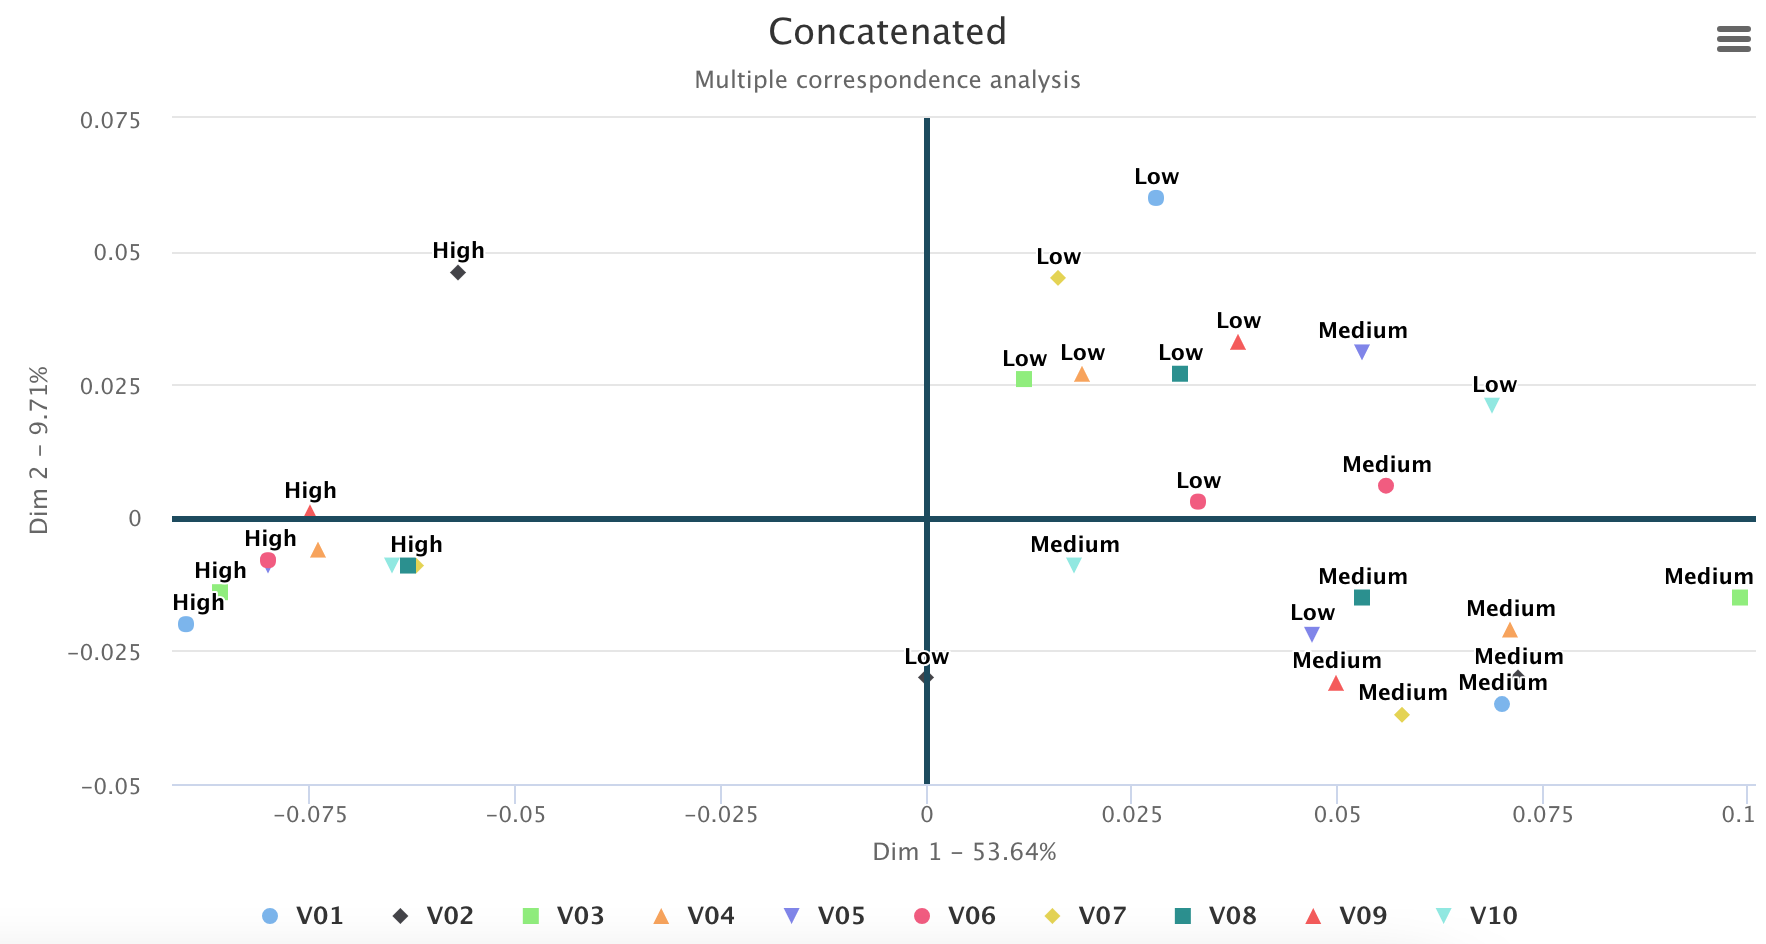
\includegraphics[width=0.9\linewidth,]{concatenated} \end{center}

\caption{Análisis de correspondencias múltiples aplicado a la tabla concatenada.}

\label{fig:concatenatedfig}
\end{figure}

Otro resultado es el MCA aplicado a una tabla específica. En este punto,
uno de los argumentos que se debe tener en cuenta es la selección de la
tabla con la que se realizará el análisis.

Al comparar los gráficos, se puede observar que la tabla del punto b
(\ref{fig:bfig}) muestra diferencias con la tabla del estado bajo
control (\ref{fig:concatenatedfig}); sin embargo, las diferencias no
llegan a ser significativas, por lo que no genera una señal de fuera de
control (\ref{fig:tdos}, punto b).

\begin{figure}[H]


\begin{center}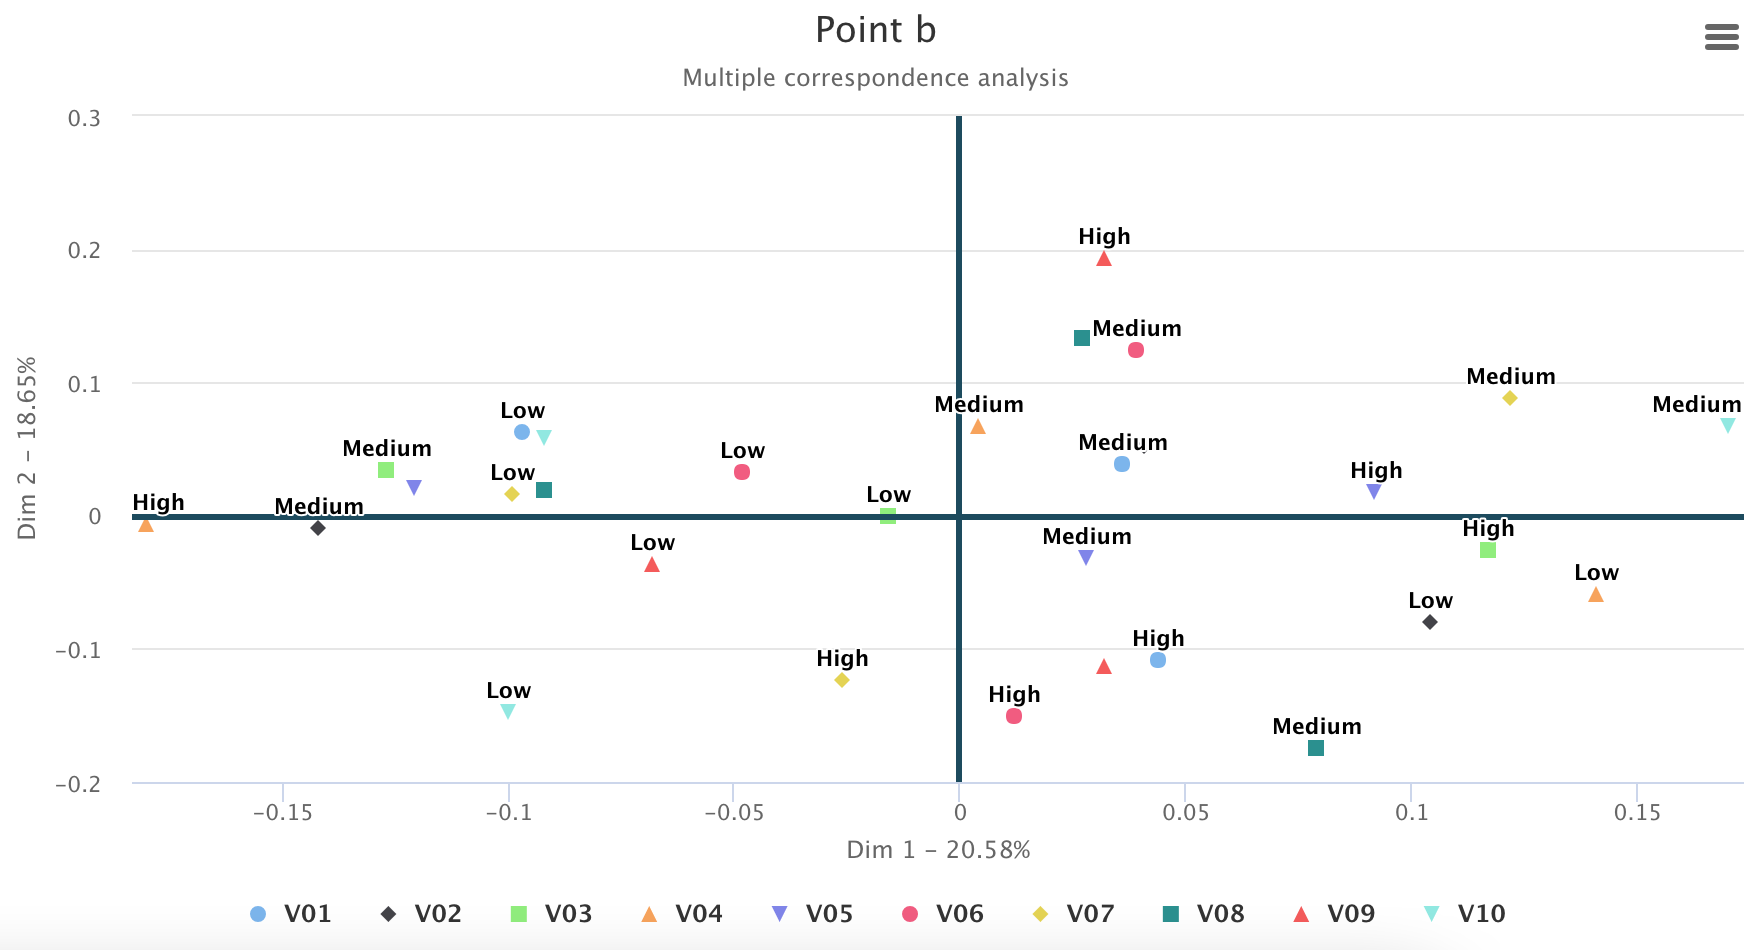
\includegraphics[width=0.9\linewidth,]{pointb} \end{center}

\caption{Análisis de correspondencias múltiples aplicado a la tabla b.}

\label{fig:bfig}
\end{figure}

La figura \ref{fig:bfig} representa el gráfico del MCA de la tabla b,
correspondiente a un momento específico del proceso monitorizado. Este
gráfico, en sus dos dimensiones, representa al 39.23\% de la
información. Es notorio que las observaciones en sus niveles \emph{alto,
medio y bajo} están distribuidas de forma aleatoria en todos los
cuadrantes del gráfico, no se puede precisar un patrón específico de
agrupación.

Lo mismo se puede decir de los puntos representados en cualquiera de las
otras tablas porque comparten la misma distribución, exceptuando la
tabla j, que fue diseñada con una distribución diferente. No obstante,
el uso del MCA de las figuras \ref{fig:bfig} y \ref{fig:concatenatedfig}
todavía no permite detectar si el proceso está o no en control. La
identificación de puntos fuera de control se puede realizar mediante la
representación gráfica del estadístico \(T^2_{med}\), como se observa en
la figura \ref{fig:tdos}.

\begin{figure}[H]


\begin{center}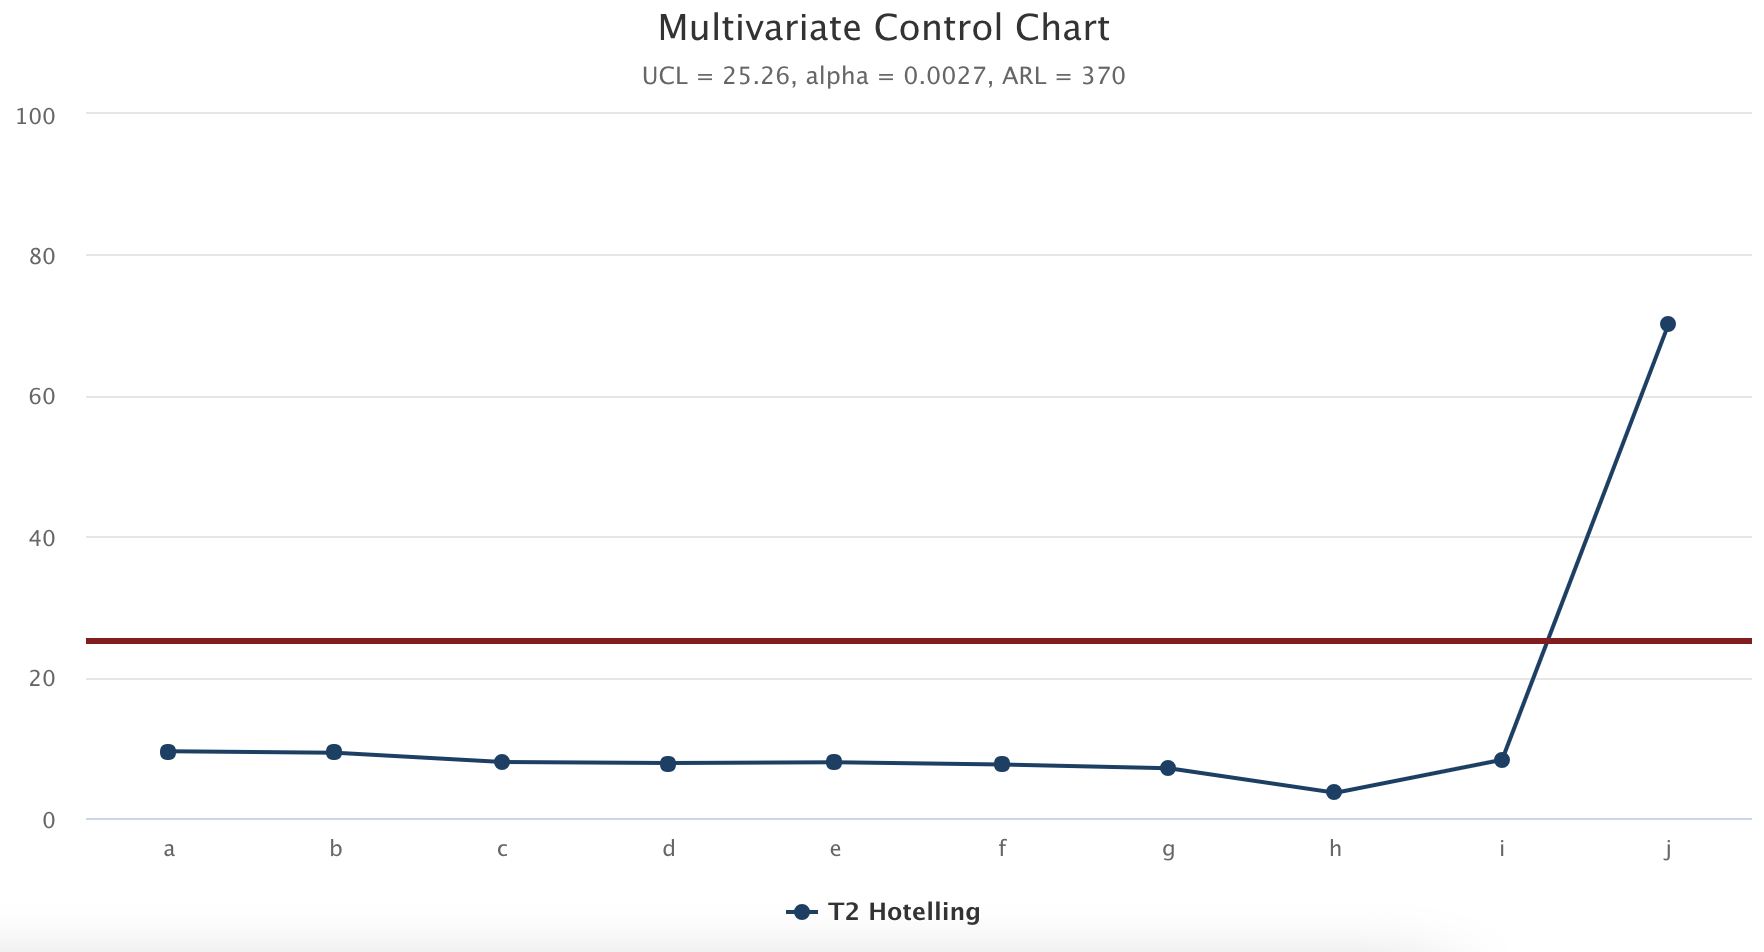
\includegraphics[width=0.9\linewidth,]{t2} \end{center}

\caption{Gráfico de control multivariante T2 Hotelling aplicable a variables cualitativas, $Datak10Contaminated$.}

\label{fig:tdos}
\end{figure}

La figura \ref{fig:tdos} presenta al gráfico de control T2Qv, basado en
el estadístico T2 de Hotelling ajustado (\(T^2_{med}\)), aplicado a la
detección de anomalías en cualquiera de las \emph{K} tablas analizadas.
Cada una de las tablas está representada por los puntos en el gráfico.
Se observa una línea horizontal que representa al límite de control
superior (UCL). El límite de control inferior (LCL) es igual a cero.

Se observa que el punto que representa a la tabla \emph{j} se ubica por
encima del límite de control superior, lo que quiere decir que se lo ha
identificado como un valor fuera de control. Por consiguiente, es
necesario analizar con detenimiento qué está pasando con los datos de la
tabla reportada, comparándolos con los de la tabla concatenada, a fin de
identificar las causas de la variación y tomar las acciones pertinentes.
Para hacer un análisis del punto fuera de control se realiza un gráfico
del MCA de la tabla \emph{j} y se lo compara con el gráfico similar de
la tabla concatenada, como se presenta en la figura
\ref{fig:comparation}.

\begin{figure}[H]


\begin{center}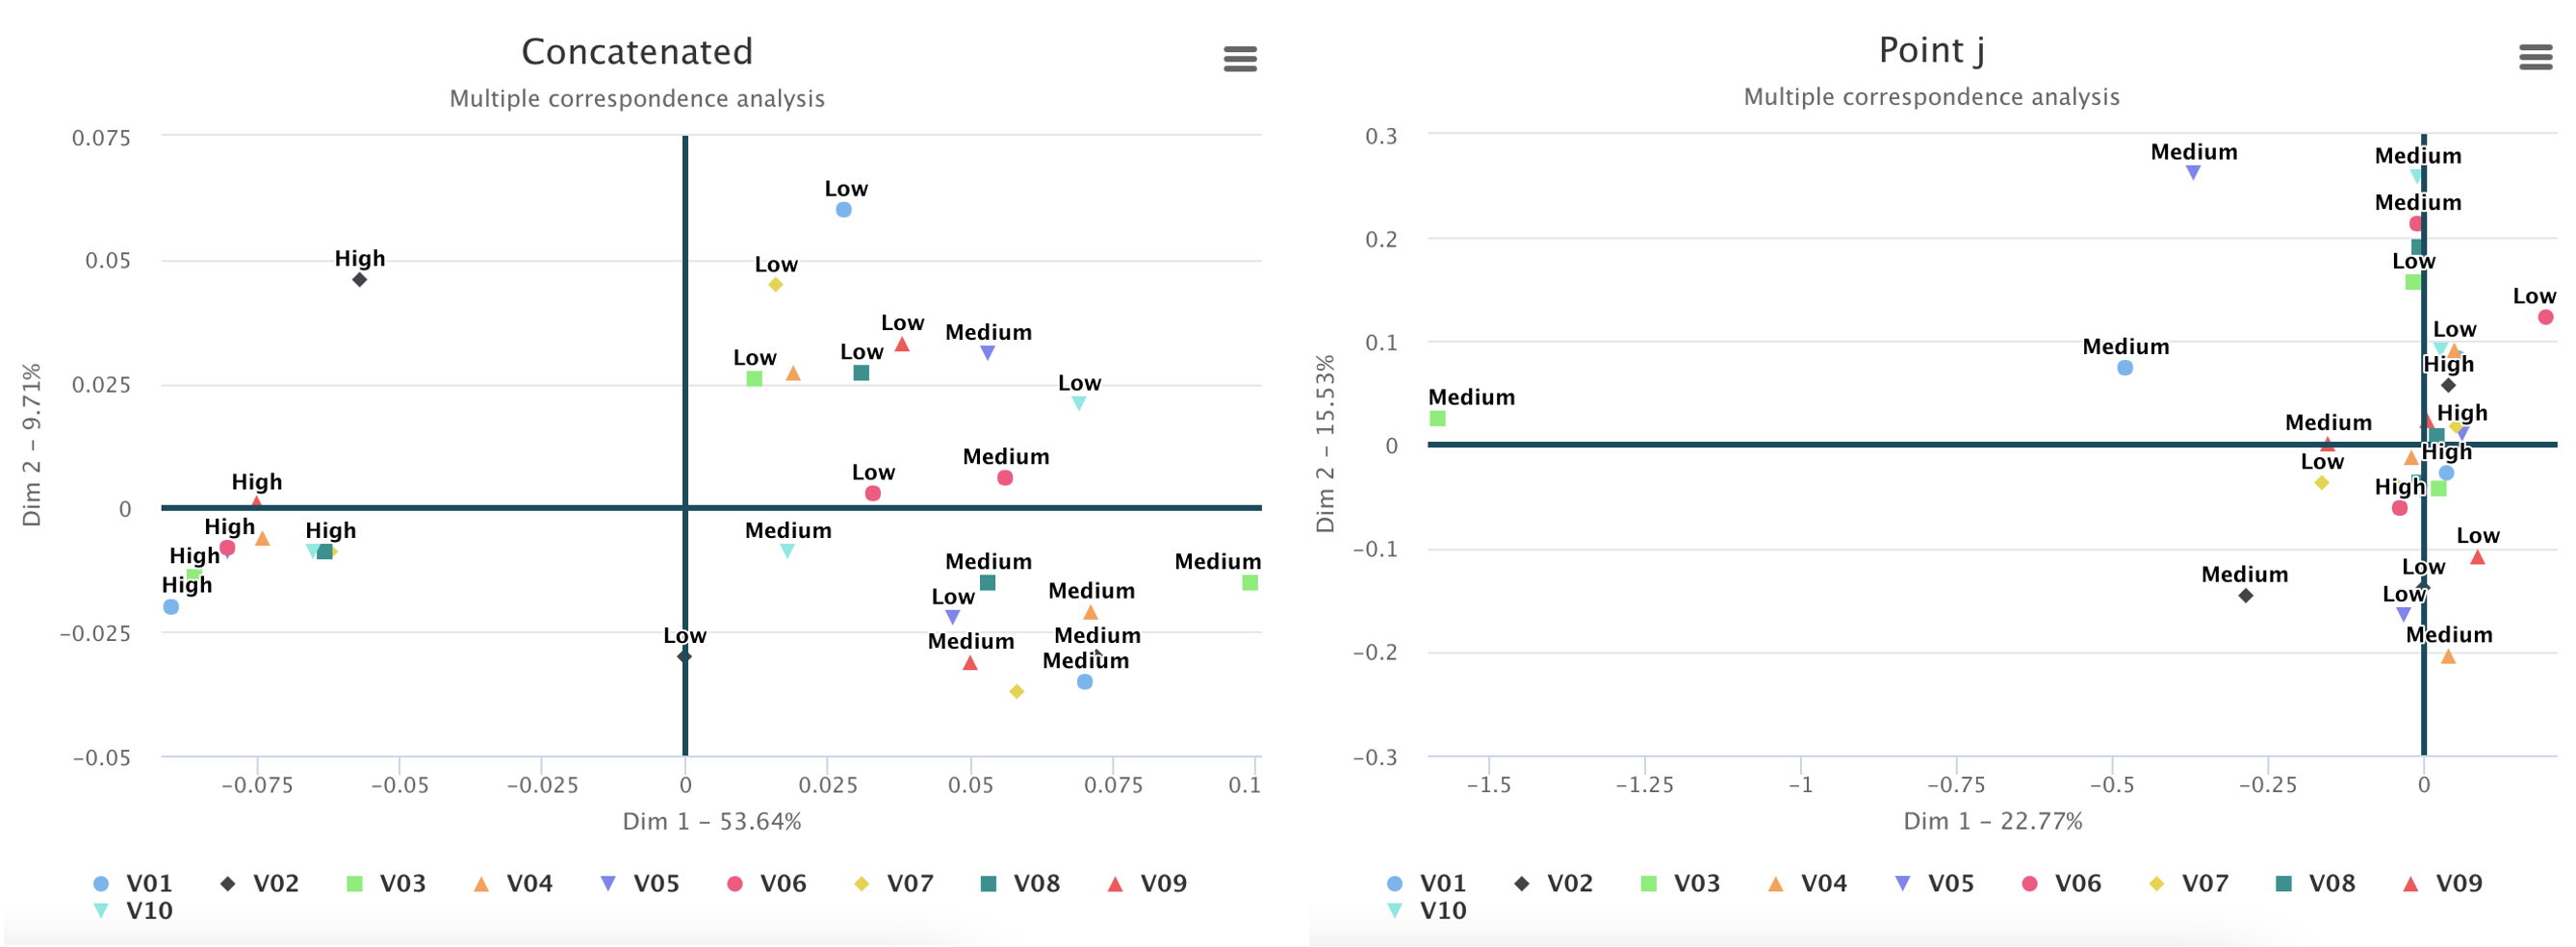
\includegraphics[width=0.9\linewidth,]{comparation} \end{center}

\caption{Gráfico de control multivariante T2 Hotelling aplicable a variables cualitativas, $Datak10Contaminated$.}

\label{fig:comparation}
\end{figure}

La figura \ref{fig:comparation} presenta la distribución de las
observaciones de las tablas concatenada y \emph{j} mediante gráficos del
MCA. El gráfico de la tabla concatenada, que sirve de referente en
control, ya se analizó en la Figura 4. El gráfico de la tabla \emph{j}
muestra una tendencia de los valores medios de las variables a ubicarse
al lado izquierdo, alejándose del centro del gráfico, lo que indica que
los valores medios son poco frecuentes. Especial atención merece la
variable 3, que registra una observación para el nivel medio con el
valor más alejado del grupo. Por el contrario, las categorías altas se
han situado en el centro, lo que significa que son muy frecuentes.

Al comparar los gráficos es evidente que la distribución de los datos en
el gráfico de la tabla \emph{j} es diferente de las distribuciones de
las demás tablas, y en especial, es diferente de la distribución de los
datos en el gráfico de la tabla concatenada, lo que explica por qué el
punto \emph{j} ha sido identificado como fuera de control en el gráfico
T2Qv. Esta diferencia se explica en la Tabla 6, que muestra la distancia
Chi cuadrado entre las observaciones de la tabla concatenada y la tabla
\emph{j}.

\begin{table}[H]
\centering
\begin{tabular}{lr}
\toprule
\multicolumn{1}{c}{\cellcolor[HTML]{FFFFFF}{\color[HTML]{000000} \textbf{Variables}}} & \multicolumn{1}{c}{\textbf{ChiSq}} \\ \midrule

\textbf{V1}                                                                             & {\color[HTML]{333333} 0.06968}      \\ 
\textbf{V2}                                                                       & {\color[HTML]{333333} 0.05010}      \\ 
\textbf{V3}                                                                       & {\color[HTML]{333333} 0.07601}      \\ 
\textbf{V4}                                                                       & {\color[HTML]{333333} 0.04982}      \\ 
\textbf{V5}                                                                       & {\color[HTML]{333333} 0.05205}      \\ 
\textbf{V6}                                                                       & {\color[HTML]{333333} 0.05603}      \\ 
\textbf{V7}                                                                       & {\color[HTML]{333333} 0.03713}      \\ 
\textbf{V8}                                                                       & {\color[HTML]{333333} 0.03702}      \\ 
\textbf{V9}                                                                       & {\color[HTML]{333333} 0.04395}      \\ 
\textbf{V10}                                                                            & {\color[HTML]{333333} 0.06179}      \\ \hline
\end{tabular}
\caption{Distancia Chi cuadrado entre las masas de columna de la tabla k y la concatenada, $Datak10Contaminated$.}

\label{tab:chiexamp}
\end{table}

Otra manera de visualizar esta información es a través de un gráfico de
barras que genera el aplicativo T2Qv (figura \ref{fig:chisqr}).

\begin{figure}[H]


\begin{center}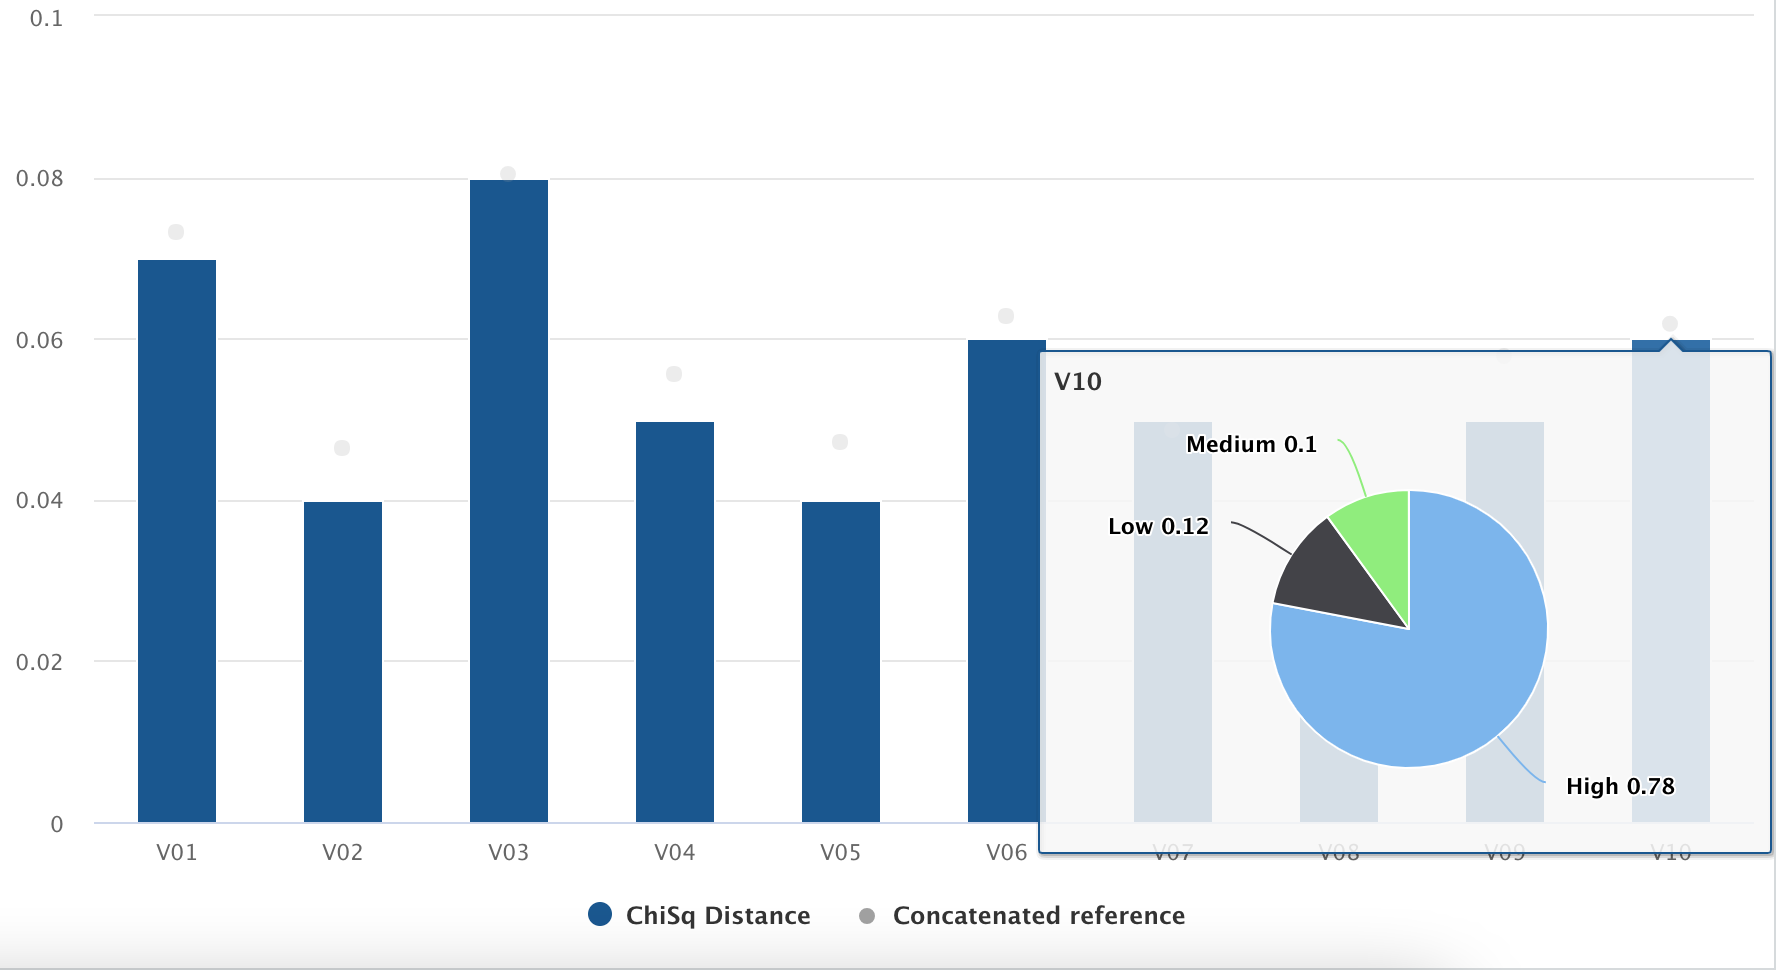
\includegraphics[width=0.9\linewidth,]{Chisqr} \end{center}

\caption{Distancia Chi cuadrado entre las masas de la tabla concatenada y las k tablas, $Datak10Contaminated$.}

\label{fig:chisqr}
\end{figure}

El gráfico de barras de la figura \ref{fig:chisqr}, expresa también la
distancia \(\chi^{2}\) entre las masas de la tabla concatenada y las de
las k tablas de la base de datos Datak10Contaminated, en este caso la j.
En la Tabla \ref{tab:chiexamp} se observa que las variables V03, V01 y
V06 manifiestan las mayores distancias Chi cuadrado entre las masas de
la tabla concatenada y la tabla j (0.07700, 0.06968, 0.05938), lo que en
la figura \ref{fig:chisqr} se representa con las barras más altas.

La interactividad de este gráfico facilita la observación de la
distribución de las categorías de las variables de la tabla analizada, y
su comparación con la distribución de las categorías de las variables en
la tabla concatenada, como se observa en la figura \ref{fig:distcomp}.

\begin{figure}[H]


\begin{center}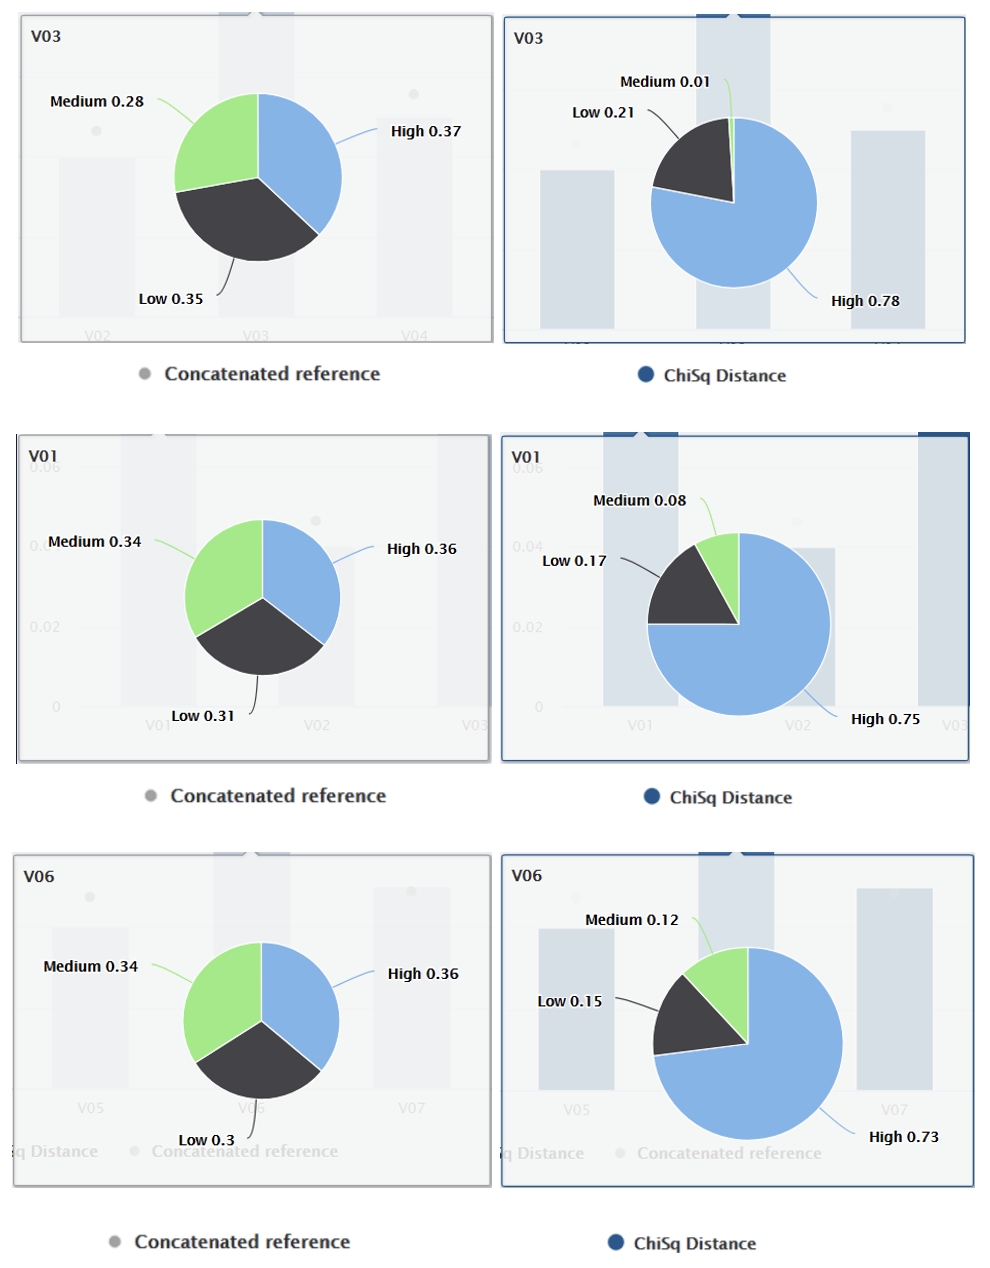
\includegraphics[width=0.9\linewidth,]{distcomp} \end{center}

\caption{Distribución de las categorías de las variables V03, V01 y V06 en la tabla Concatenada y la tabla $j$ en el aplicativo T2Qv.}

\label{fig:distcomp}
\end{figure}

La figura 9 presenta, en gráficos circulares, la distribución de las
categorías de las variables V03, V01 y V06, que registraron mayores
distancias Chi cuadrado entre las masas de la tabla concatenada y la
tabla \emph{j}. Los gráficos que corresponden a la tabla concatenada
presentan sectores con áreas equivalentes entre sí, lo que se explica
por la distribución uniforme de las variables, mientras que, los de la
tabla \emph{j} muestran áreas con tamaños variados, donde la categoría
\emph{High} tiene una frecuencia relativa alta en los tres casos, y
\emph{Low}, baja frecuencia. Al comparar estos gráficos se hace evidente
que la distribución de las categorías presenta grandes diferencias entre
la tabla concatenada y la tabla \emph{j}. El comportamiento de estas
variables tiene mayor incidencia en el desplazamiento de la tendencia
central del proceso que, al final, lo lleva a un estado fuera de
control. Sin embargo, al tratarse de un contexto multivariante, todas
las variables contribuyen en mayor o menor medida a explicar el
comportamiento del proceso, de manera que la salida de control no se
puede atribuir a la acción individual de una variable, o a la acción por
separado de un grupo de ellas, sino al efecto combinado de las variables
correlacionadas.

\hypertarget{anuxe1lisis-de-sensibilidad}{%
\section{Análisis de sensibilidad}\label{anuxe1lisis-de-sensibilidad}}

Como se ha mencionado, en el gráfico T2Qv un punto fuera de control se
interpreta como una tabla (\(k_i\)) que incluye una cantidad o una
proporción de variables contaminadas. En estos casos, se espera que los
puntos en el gráfico T2Qv generalicen el comportamiento de estas
diferencias en su distribución y así se supere el límite de control
superior (UCL). La ubicación de este límite de control varía en función
del número de dimensiones que se representen, así, cuando es alto se
logra un desempeño óptimo, mientras que, se introduce inestabilidad y se
pierde confiabilidad en los resultados al disminuir el número de
dimensiones que se pueden representar.

El gráfico de control propuesto es capaz de detectar un punto fuera de
control, aún con un bajo número de variables contaminadas, cuando se
trabaja con un alto número de dimensiones. Se recomienda \(p - 1\), tal
que \emph{p} es el número total de dimensiones de la matriz inicial
(Tabla \ref{tab:inicial}). Cuando se disminuye el número de dimensiones
también disminuye la altura del límite de control superior (UCL), en
consecuencia, se incrementa el número de puntos fuera de control, aunque
no necesariamente las variables expresen diferencias significativas en
su valores, crece la probabilidad de obtener error tipo I.

Por consiguiente, la pregunta que surge es hasta cuántas dimensiones se
puede disminuir en el análisis sin perder confiabilidad en el resultado.
La importancia de esta pregunta radica en la necesidad de disponer un
gráfico confiable, que identifique puntos fuera de control aún si se ha
aplicado a los datos una técnica de una reducción de dimensiones, sin
caer en casos de falso positivo.

\begin{figure}[H]


\begin{center}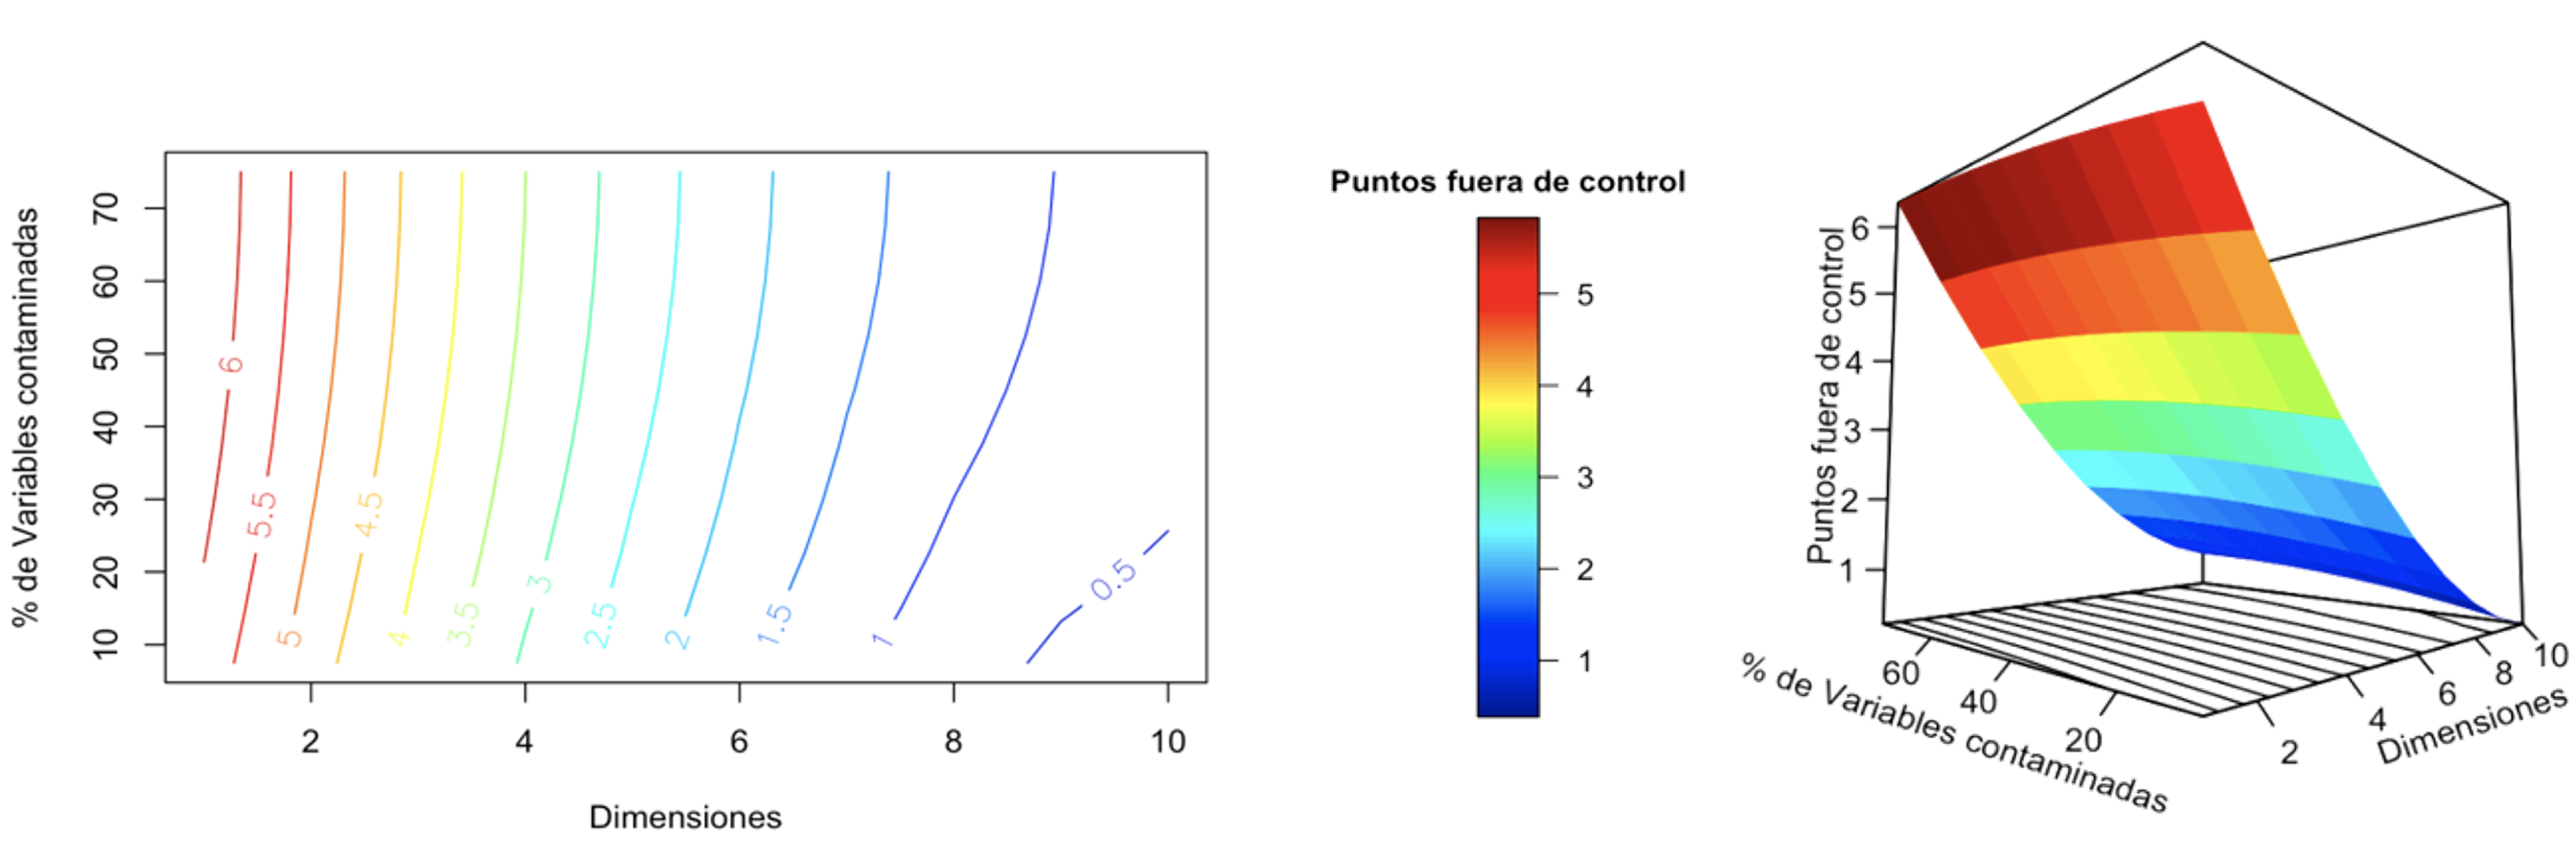
\includegraphics[width=0.9\linewidth,]{sensibilidad} \end{center}

\caption{Curvas de nivel y superficie de respuesta obtenidas con el gráfico T2Qv.}
\label{fig:sensibilidad}
\end{figure}

El análisis de sensibilidad utiliza curvas de nivel y superficies de
respuesta (figura \ref{fig:sensibilidad}) para representar el número de
puntos fuera de control, considerando el porcentaje de variables
contaminadas de la \emph{ki} tabla y el número de dimensiones
representadas. Los datos de prueba utilizados en el modelo se registran
en 10 tablas, cada una de ellas incluye 10 variables y cada variable
tiene tres categorías: \emph{High, Medium} y \emph{Low} La tabla 10 (o
tabla j) tiene una distribución diferente de las demás, esta es la tabla
contaminada.

Se observa que el modelo es capaz de identificar un punto fuera de
control trabajando con \emph{p} -- 1 dimensiones (9), aún con un
porcentaje bajo de variables contaminadas. Cuando el número de
dimensiones disminuye a \emph{p} -- 2 (8) y el porcentaje de variables
contaminadas es cercano a 100\%, detecta correctamente 1 punto fuera de
control. Se observa además que cuando el número de dimensiones es menor
se pierde estabilidad y se mitiga la potencia de la prueba. En
consecuencia, el análisis de sensibilidad ratifica que el gráfico de
control T2Qv tiene un buen rendimiento cuando trabaja con altas
dimensiones.

\hypertarget{discusiuxf3n}{%
\section{Discusión}\label{discusiuxf3n}}

En el control estadístico de procesos todavía no son muchas las
propuestas publicadas sobre gráficos de control para variables
cualitativas. Las diferencias entre procedimientos para la determinación
de los estadísticos y los gráficos de control en este campo hacen
difícil su comparación.

El gráfico de control T2Qv, que se presenta en este artículo, aplica
MCA, técnica de análisis multivariante que identifica estructuras
latentes que subyacen en el conjunto de datos cualitativos y que
involucra una reducción de dimensiones, en consecuencia, desde el
comienzo se requiere una tabla de datos con \emph{p} variables (\emph{p}
\textgreater{} 3) dicotómicas o politómicas. Vale recordar que el
análisis de sensibilidad determinó que esta propuesta tiene un buen
rendimiento cuando trabaja con altas dimensiones y que a bajas
dimensiones pierde estabilidad. De esta manera, mientras que en el
ejemplo con datos simulados \emph{Datak10Contaminated} que se presenta
en esta investigación, el T2Qv analiza el comportamiento de 10
variables, en varios estudios revisados, los casos de aplicación
analizan sólo dos o tres, lo que conduciría a la aplicación de un
análisis de correspondencias simple, no múltiple. En consecuencia, estos
casos no podrían ser tratados con el T2Qv.

Como ejemplos se señala la Combinación lineal óptima de variables
Poisson para el SPC multivariados, de \citet{epprecht2013optimal}, cuyo
caso de aplicación registrado en su publicación analiza dos variables
relacionadas con el conteo de defectos en la producción de jarrones de
cerámica. El gráfico GMDS de \citet{raza2019design} fue ejemplificado
con un conjunto de datos de telecomunicaciones, tomado de
\citet{jiang2002process}, que consta de sólo dos variables. El gráfico
de control multivariante, desarrollado por
\citet{pastuizaca2015multivariate}), para \emph{p} características de
calidad de atributos correlacionadas, que aplica teoría difusa, hace un
análisis de dos tablas tomadas de publicaciones de
\citet{taleb2009control} y \citet{taleb2006multivariate}, la primera con
tres variables relacionadas con la comida congelada, y la segunda, con
tres variables sobre la producción de porcelana.

Otra de las características del gráfico T2Qv es que cada muestra es un
grupo constituido por un conjunto de individuos, una tabla. El ejemplo
de datos simulados \emph{Datak10Contaminated} incluye un conjunto de 10
tablas y 11 variables, cada tabla es una muestra, está formada por 100
observaciones y aparece representada como un punto en el gráfico T2 de
Hotelling.

En publicaciones de varios autores se puede constatar que en sus
ejemplos de aplicación se analiza una sola tabla, de dimensiones
\emph{n} (filas) x \emph{p} (variables), donde cada ni fila es una
muestra. Por ejemplo, el gráfico de control MNP, de
\citet{lu1998control} contiene en su artículo una tabla de datos
simulados de 30 muestras, donde cada una de ellas es un único individuo
(objeto) que registra el conteo de defectos para tres características de
la calidad. Asimismo, la ejemplificación que \citet{chiu2007}
presentaron de su gráfico de control MP se hizo con una tabla de datos
simulados de 26 muestras, donde cada muestra representa a un individuo
al que se le registra el \emph{D} número de defectos o no conformidades
asociadas a tres características de calidad.

En el gráfico de control T2Qv que se presenta en este artículo, cada uno
de los individuos (filas) que conforman las diferentes nuestras pueden
tener distintas configuraciones en función de las categorías de las
variables.

Por el contrario, otros autores que han investigado sobre gráficos de
control multivariante para datos de atributos, aunque en su análisis
consideran varias características de calidad, al final clasifican a cada
individuo por una sola de las variables analizadas. Es el caso de
\citet{ranjan2008multivariate}, cuya propuesta se demuestra con un caso
de aplicación que controla 7 características de calidad en 24 muestras
cuyo tamaño varía entre 20 y 404 individuos. Las variables responden a 6
tipos de defectos de la pintura en la cubierta de ventiladores de techo:
cobertura deficiente, desbordamiento, defecto de empanada, burbujas,
defectos de pintura, defectos de pulido. La séptima característica es la
ausencia de defectos. A cada individuo se lo clasifica por su defecto
más predominante, por consiguiente, en su registro sólo aparece un tipo
de defecto o ausencia de defectos, lo que resulta en una pérdida de
información sobre el efecto combinado de las variables sobre el proceso.

Los gráficos de control que incorporan técnicas multivariantes dirigen
su aplicación al análisis de variables categóricas y numéricas en una
misma tabla de datos. Por ejemplo, el gráfico de control PCA Mix
\citep{Ahsan2020} convierte las variables de atributo en ficticias y las
trata junto con las variables continuas, para generar una matriz Kernel
y calcular las componentes principales. Una debilidad de esta propuesta
está en que su rendimiento disminuye en presencia de proporciones
extremadamente desequilibradas de las categorías de variables
cualitativas, situación que se propone corregir aplicando el método
Kernel PCA (KPCA), una versión no lineal del PCA convencional que modela
datos de distribuciones no gaussianas.

Estos ajustes al rendimiento corresponden a una fase II de los gráficos
de control, con miras a su optimización. El T2Qv es un gráfico de
control de procesos multivariantes que maneja variables cualitativas en
fase I, en consecuencia, no se ha considerado aún la evaluación de su
eficiencia, por lo que ambos gráficos no son comparables. Sin embargo,
es precisamente el cambio en la distribución de las categorías de las
variables, de balanceada a desequilibrada, o viceversa, lo que detecta
el T2Qv como punto fuera de control.

Una propuesta interesante es la de \citet{Saltos2020}, quienes utilizan
el concepto de profundidad para el análisis de una tabla de datos en el
campo de la educación, pero, al final la representación del rendimiento
académico es univariante y se realiza mediante una carta de control r.
El ACM, siendo una técnica factorial que trabaja en términos de
asociación de variabilidad, hace que la información común a todos los
casos, o a la gran mayoría, sea estable y por lo tanto no aparezca en
los ejes primarios, en el mejor de los casos se concentra en el origen
del gráfico. De hecho en el aplicativo T2Qv, cuando una categoría de
alguna variable es constante en una tabla de la base de datos, se
reporta un error que impide la ejecución, pero, si hay por lo menos un
caso diferente, éste se representaría como un punto muy alejado en algún
extremo del gráfico, mientras que la categoría que registre la mayor
frecuencia se ubicaría como un punto en el centro. Esto podría
constituir una característica propia de la naturaleza del ACM, que sólo
puede representar parcialmente la variabilidad de la información en sus
dos dimensiones.

Para corregir este problema, la metodología propuesta en esta
investigación, aunada a la técnica del ACM, utiliza el gráfico T2Qv que,
como queda establecido en el análisis de sensibilidad, funciona mejor
con la mayor cantidad de dimensiones, es decir, recoge la mayor cantidad
de variabilidad para identificar el punto (la tabla punto) fuera de
control. Además, un análisis comparativo posterior establece la
distancia \(\chi^{2}\) entre los valores reportados por las categorías
de la tabla concatenada y la tabla punto para una variable específica y
la representa en un gráfico de barras, lo que permite la identificación
de las variables que más están produciendo anomalías. Finalmente, el
aplicativo facilita la comparación de la distribución de las categorías
de la variable analizada en la tabla punto y la concatenada a través de
un recurso gráfico interactivo que utiliza gráficos de sectores.

Una oportunidad para futuras investigaciones relacionadas con el control
multivariante para variables cualitativas podría ser la optimización del
gráfico, con un límite de control que se ajuste a los parámetros
específicos del análisis, llevándolo hasta a una fase II del control
estadístico de procesos. Otra oportunidad sería el desarrollo de una
metodología que vaya más allá del análisis de la primera dimensión
latente, que es lo que hace la propuesta de esta investigación cuando
aplica ACM. Podría ser viable la incorporación, por ejemplo, de un Meta
Biplot \citep{galindojk} , técnica que analiza de forma cruzada todas
las dimensiones latentes.

\hypertarget{conclusiones}{%
\section{Conclusiones}\label{conclusiones}}

En este artículo se ha presentado una herramienta para control
estadístico de procesos multivariantes que realiza un análisis de los
datos cualitativos, al que se ha denominado Gráfico de control T2Qv,
basado en un Análisis de Correspondencias Múltiples. Las coordenadas
normalizadas, se representan mediante el gráfico T2 de Hotelling
robusto.

Para facilitar la difusión y aplicación del método propuesto, se ha
desarrollado un paquete estadístico computacional reproducible en R,
denominado T2Qv y disponible en CRAN, que permite visualizar los
resultados de forma plana o interactiva, además, presenta un panel Shiny
que contiene todas las funciones integradas en un mismo espacio.

Esta propuesta genera un gráfico del MCA de la tabla concatenada, que
sirve de referente para comparar otros gráficos del MCA de las tablas
que hayan sido identificadas como puntos fuera de control en el gráfico
de Hotelling. Allí se puede verificar qué categorías de las variables
han tenido variaciones en su ubicación en ambos gráficos, que pueden
estar provocando cambios en la centralidad del proceso y ocasionando el
estado de fuera de control.

Para facilitar la interpretación del comportamiento de las variables se
realiza un análisis de la distancia Chi cuadrado entre las categorías de
la tabla concatenada y de las tablas reportadas como fuera de control,
analítica y gráficamente, incluyendo gráficos interactivos que presentan
la distribución porcentual de las categorías de las variables
analizadas.

En un contexto multivariante, todas las variables contribuyen en mayor o
menor medida a explicar el comportamiento del proceso, de manera que la
salida de control no se puede atribuir a la acción individual de una
variable, o a la acción por separado de un grupo de ellas, sino al
efecto combinado de variables correlacionadas. Por eso es preciso el
enfoque multivariante en el control de procesos estadísticos.

El análisis de sensibilidad determinó que el gráfico de control T2Qv
tiene un buen rendimiento cuando trabaja con altas dimensiones, pero,
pierde estabilidad a bajas dimensiones.

En el control estadístico de procesos multivariantes para variables
cualitativas todavía no son muchas las propuestas publicadas. Las
diferencias entre procedimientos para la determinación de los
estadísticos y los gráficos de control en este campo hacen difícil su
comparación.

El gráfico de control T2Qv atiende la necesidad de un gráfico
multivariante de control estadístico para variables cualitativas en
procesos sociales, donde es muy común el uso de variables nominales y
ordinales.

% %%%%%%%%%%%%%%%%%%%%%%%%%%%%%%%%%%%%%%%%%%
% %% optional
% \supplementary{The following are available online at www.mdpi.com/link, Figure S1: title, Table S1: title, Video S1: title.}
%
% % Only for the journal Methods and Protocols:
% % If you wish to submit a video article, please do so with any other supplementary material.
% % \supplementary{The following are available at www.mdpi.com/link: Figure S1: title, Table S1: title, Video S1: title. A supporting video article is available at doi: link.}

\vspace{6pt}

%%%%%%%%%%%%%%%%%%%%%%%%%%%%%%%%%%%%%%%%%%

%%%%%%%%%%%%%%%%%%%%%%%%%%%%%%%%%%%%%%%%%%

%%%%%%%%%%%%%%%%%%%%%%%%%%%%%%%%%%%%%%%%%%

%%%%%%%%%%%%%%%%%%%%%%%%%%%%%%%%%%%%%%%%%%
%% optional


%%%%%%%%%%%%%%%%%%%%%%%%%%%%%%%%%%%%%%%%%%
% Citations and References in Supplementary files are permitted provided that they also appear in the reference list here.

%=====================================
% References, variant A: internal bibliography
%=====================================
%\reftitle{References}
%\begin{thebibliography}{999}
% Reference 1
%\bibitem[Author1(year)]{ref-journal}
%Author1, T. The title of the cited article. {\em Journal Abbreviation} {\bf 2008}, {\em 10}, 142--149.
% Reference 2
%\bibitem[Author2(year)]{ref-book}
%Author2, L. The title of the cited contribution. In {\em The Book Title}; Editor1, F., Editor2, A., Eds.; Publishing House: City, Country, 2007; pp. 32--58.
%\end{thebibliography}

% The following MDPI journals use author-date citation: Arts, Econometrics, Economies, Genealogy, Humanities, IJFS, JRFM, Laws, Religions, Risks, Social Sciences. For those journals, please follow the formatting guidelines on http://www.mdpi.com/authors/references
% To cite two works by the same author: \citeauthor{ref-journal-1a} (\citeyear{ref-journal-1a}, \citeyear{ref-journal-1b}). This produces: Whittaker (1967, 1975)
% To cite two works by the same author with specific pages: \citeauthor{ref-journal-3a} (\citeyear{ref-journal-3a}, p. 328; \citeyear{ref-journal-3b}, p.475). This produces: Wong (1999, p. 328; 2000, p. 475)

%=====================================
% References, variant B: external bibliography
%=====================================
\reftitle{References}
\externalbibliography{yes}
\bibliography{mybibfile.bib}

%%%%%%%%%%%%%%%%%%%%%%%%%%%%%%%%%%%%%%%%%%
%% optional

%% for journal Sci
%\reviewreports{\\
%Reviewer 1 comments and authors’ response\\
%Reviewer 2 comments and authors’ response\\
%Reviewer 3 comments and authors’ response
%}

%%%%%%%%%%%%%%%%%%%%%%%%%%%%%%%%%%%%%%%%%%
\end{document}
